% ============================================================================
%  RAPPORT D'AUDIT DU GSE IRCANTEC
%  Nexialog Consulting — Pôle Risques Financiers & Actuariat
%  Mise en forme : charte Nexialog v2 (skill nexialog-note-technique-latex)
%  Compilation : pdflatex (x2) ou latexmk -pdf
%  Pré-requis polices : Montserrat + Source Sans Pro (cf. SKILL.md du skill)
% ============================================================================
\documentclass[11pt,a4paper]{article}

% --------- ENCODAGE & POLICES (charte Nexialog v2) --------------------------
% Texte courant  -> Source Sans Pro (substitut libre proche de Segoe UI)
% Titres / sf    -> Montserrat (via \sffamily)
\usepackage[utf8]{inputenc}
\usepackage[T1]{fontenc}
\usepackage[default]{sourcesanspro}
\usepackage{montserrat}
\usepackage{microtype}
\usepackage{cmap}
\frenchspacing
\providecommand{\og}{\guillemotleft~}
\providecommand{\fg}{~\guillemotright}
\providecommand{\ier}{\textsuperscript{er}}

% --------- MISE EN PAGE -----------------------------------------------------
\usepackage[a4paper,top=32mm,bottom=22mm,left=25mm,right=25mm,
            headheight=19mm,headsep=6mm]{geometry}
% Charte v2 : pas de \setstretch ni de \parskip — interligne et espacement
% des paragraphes laissés aux valeurs LaTeX par défaut (paragraphes indentés),
% conformément au template du skill nexialog-note-technique-latex.

% --------- COULEURS : palette officielle Nexialog v2 ------------------------
\usepackage{xcolor,colortbl}
\definecolor{nxnavy}{HTML}{002060}        % NexialogBlue (bleu principal)
\definecolor{nxred}{HTML}{B10031}         % NexialogRed (rouge accents/alertes)
\definecolor{nxteal}{HTML}{409ABB}        % NexialogTeal
\definecolor{nxslate}{HTML}{223E55}       % NexialogSlate
\definecolor{nxgray}{HTML}{9A999E}        % NexialogGray
\definecolor{nxlightgray}{HTML}{D0D1D4}   % NexialogLightGray
\definecolor{nxoffwhite}{HTML}{F2F2F2}    % NexialogOffWhite
\definecolor{nxgreen}{HTML}{2E7D32}       % NexialogGreen (réservé tableaux)
\definecolor{nxorange}{HTML}{F57C00}      % NexialogOrange (réservé tableaux)
\definecolor{nxlightblue}{HTML}{E6ECF7}   % bleu très clair (encadrés)
% Alias des noms hérités du document source -> palette v2
% (compatibilité des tableaux, encadrés et titres déjà rédigés ; aucune
%  retouche du corps n'est nécessaire).
\colorlet{nexnavy}{nxnavy}
\colorlet{nexred}{nxred}
\colorlet{nexgrey}{nxgray}
\colorlet{nexlight}{nxoffwhite}
\colorlet{nexgreen}{nxgreen}
\colorlet{tabborder}{nxlightgray}
\colorlet{nexbrick}{nxred}
\colorlet{nexbrickbg}{nxoffwhite}

% --------- PACKAGES FONCTIONNELS --------------------------------------------
\usepackage{amsmath,amssymb}
\usepackage{bm}
\usepackage{graphicx}
\usepackage{eurosym}
\usepackage{textcomp}
\usepackage{booktabs}
\usepackage{tabularx}
\usepackage{longtable}
\usepackage{array}
\usepackage{multirow}
\usepackage{float}
\usepackage{ragged2e}
\usepackage{caption}
\usepackage{subcaption}
\usepackage{tikz}
\usetikzlibrary{positioning, arrows.meta, calc}
\usepackage{enumitem}
\usepackage{fancyhdr,lastpage}
\usepackage{titlesec}
\usepackage[hyperref]{etoc}      % TOC sur-mesure + liens (charge hyperref)
\usepackage[most]{tcolorbox}
\usepackage{needspace}
\usepackage{etoolbox}
\usepackage{xurl}               % coupure des URLs longs
\usepackage{hyperref}

% Listes : bullets désindentés (charte v2, BCG/McKinsey-like), réglage global.
\setlist{leftmargin=*, labelindent=0pt, itemsep=2pt, topsep=4pt}

% --------- EN-TÊTE / PIED (charte v2 : logo + filet fin) --------------------
\pagestyle{fancy}
\fancyhf{}
\fancyhead[L]{\parbox[c][14mm][c]{52mm}{\includegraphics[height=12mm]{logo_nexialog.pdf}}}
\fancyhead[R]{\parbox[c][14mm][c]{110mm}{\raggedleft\small\textcolor{nxgray}{Audit du GSE IRCANTEC~~\textbar~~\textit{Confidentiel}}}}
\fancyfoot[L]{\footnotesize\textcolor{nxgray}{\copyright~Nexialog Consulting --- 2026~~\textbar~~[Réf. mission]}}
\fancyfoot[R]{\footnotesize Page \thepage~/~\pageref{LastPage}}
\renewcommand{\headrulewidth}{0pt}
\renewcommand{\footrulewidth}{0.3pt}
\renewcommand{\footrule}{\hbox to\headwidth{\color{nxlightgray}\leaders\hrule height \footrulewidth\hfill}}

% --------- STYLES DE SECTION (Montserrat navy, charte v2) -------------------
% \sffamily force Montserrat. Hiérarchie portée par la taille (pas de filet).
\titleformat{\section}{\sffamily\Large\bfseries\color{nxnavy}}{\thesection.}{0.5em}{}
\titleformat{\subsection}{\sffamily\large\bfseries\color{nxnavy}}{}{0em}{\thesubsection.~}
\titleformat{\subsubsection}{\sffamily\normalsize\bfseries\color{nxnavy}}{}{0em}{\thesubsubsection.~}

% --------- TABLE DES MATIÈRES via etoc (charte v2) --------------------------
% H1 rouge Nexialog, H2/H3 bleu navy, le tout en Montserrat, liens cliquables.
\etocsetstyle{section}
  {}{}
  {\par\noindent\sffamily\large\bfseries%
   \textcolor{nxred}{\etocname}\hfill\textcolor{nxred}{\etocpage}%
   \par\medskip}
  {}
\etocsetstyle{subsection}
  {}{}
  {\par\noindent\hspace*{5mm}\sffamily\normalsize\mdseries%
   \textcolor{nxnavy}{\etocname}\hfill\textcolor{nxnavy}{\etocpage}%
   \par\vspace{6pt}}
  {}
\etocsetstyle{subsubsection}
  {}{}
  {\par\noindent\hspace*{10mm}\sffamily\small\mdseries%
   \textcolor{nxnavy}{\etocname}\hfill\textcolor{nxnavy}{\etocpage}%
   \par\vspace{5pt}}
  {}
\etocsettocstyle{}{}

% --------- ANTI-ORPHELINS (titres) -----------------------------------------
\pretocmd{\section}{\needspace{6\baselineskip}}{}{}
\pretocmd{\subsection}{\needspace{5\baselineskip}}{}{}
\pretocmd{\subsubsection}{\needspace{4\baselineskip}}{}{}

% --------- ENCADRÉS -- charte v2 (sans cadre, titre intégré Montserrat) -----
\tcbuselibrary{skins,breakable}

% 5 encadrés standard de la charte v2 (disponibles pour la note)
\newtcolorbox{definitionbox}[1][]{
  enhanced, breakable,
  colback=nxlightblue, frame hidden, boxrule=0pt, arc=3pt,
  before skip=4mm, after skip=3mm,
  left=4mm, right=4mm, top=3mm, bottom=3mm
}
\newtcolorbox{exemplebox}[1][Exemple]{
  enhanced, breakable,
  colback=nxoffwhite, frame hidden, boxrule=0pt, arc=3pt,
  fonttitle=\sffamily\bfseries\color{nxnavy}, title=#1,
  detach title, before upper={\tcbtitle\par\nobreak\medskip\nobreak},
  before skip=4mm, after skip=3mm,
  left=4mm, right=4mm, top=3mm, bottom=3mm
}
\newtcolorbox{insightbox}[1][Point clé]{
  enhanced, breakable,
  colback=nxoffwhite, frame hidden, boxrule=0pt, arc=3pt,
  fonttitle=\sffamily\bfseries\color{nxred}, title=#1,
  detach title, before upper={\tcbtitle\par\nobreak\medskip\nobreak},
  before skip=4mm, after skip=3mm,
  left=4mm, right=4mm, top=3mm, bottom=3mm
}
\newtcolorbox{mabox}[1][]{
  enhanced, breakable,
  colback=nxlightblue, frame hidden, boxrule=0pt, arc=3pt,
  fonttitle=\sffamily\bfseries\color{nxnavy}, title=#1,
  detach title, before upper={\tcbtitle\par\nobreak\medskip\nobreak},
  before skip=4mm, after skip=3mm,
  left=4mm, right=4mm, top=3mm, bottom=3mm
}
\newtcolorbox{macbox}[1][]{
  enhanced, breakable,
  colback=nxoffwhite, frame hidden, boxrule=0pt, arc=3pt,
  fonttitle=\sffamily\bfseries\color{nxnavy!70!white}, title=#1,
  detach title, before upper={\tcbtitle\par\nobreak\medskip\nobreak},
  before skip=4mm, after skip=3mm,
  left=4mm, right=4mm, top=3mm, bottom=3mm
}

% Encadrés propres au document source, restylés selon la charte v2 :
% auditbox -> recommandation / point d'attention (titre rouge intégré)
\newtcolorbox{auditbox}{
  enhanced, breakable,
  colback=nxoffwhite, frame hidden, boxrule=0pt, arc=3pt,
  fonttitle=\sffamily\bfseries\color{nxred},
  title={Recommendation - Point d'attention},
  detach title, before upper={\tcbtitle\par\nobreak\medskip\nobreak},
  before skip=4mm, after skip=3mm,
  left=4mm, right=4mm, top=3mm, bottom=3mm
}
% minorrecbox -> recommandation mineure (titre navy intégré, fond bleu clair)
\newtcolorbox{minorrecbox}{
  enhanced, breakable,
  colback=nxlightblue, frame hidden, boxrule=0pt, arc=3pt,
  fonttitle=\sffamily\bfseries\color{nxnavy},
  title={Recommandation mineure},
  detach title, before upper={\tcbtitle\par\nobreak\medskip\nobreak},
  before skip=4mm, after skip=3mm,
  left=4mm, right=4mm, top=3mm, bottom=3mm
}

% Anti-orphelins sur les encadrés
\BeforeBeginEnvironment{definitionbox}{\needspace{5\baselineskip}}
\BeforeBeginEnvironment{exemplebox}{\needspace{5\baselineskip}}
\BeforeBeginEnvironment{insightbox}{\needspace{5\baselineskip}}
\BeforeBeginEnvironment{mabox}{\needspace{4\baselineskip}}
\BeforeBeginEnvironment{macbox}{\needspace{4\baselineskip}}
\BeforeBeginEnvironment{auditbox}{\needspace{5\baselineskip}}
\BeforeBeginEnvironment{minorrecbox}{\needspace{4\baselineskip}}

% --------- COMMANDES & STYLES DE TABLEAUX (du document, restylés v2) --------
\newcolumntype{P}[1]{>{\RaggedRight\arraybackslash}p{#1}}
\newcolumntype{R}{>{\raggedright\arraybackslash}X}   % colonne X ragged (tableaux de paramètres)
% Charte v2 : règles booktabs par défaut (noires), interligne de tableau 1.4
% (cf. rapport_Audit_GSE_CDC_Phase1, skill nexialog-note-technique-latex).
\renewcommand{\arraystretch}{1.4}
% En-tête de tableau sur fond navy (texte blanc, Montserrat)
\newcommand{\thead}[1]{\textcolor{white}{\sffamily\bfseries\small #1}}
% En-tête de tableau sur fond clair / booktabs (texte navy, Montserrat)
\newcommand{\tablehead}[1]{\textcolor{nxnavy}{\sffamily\bfseries\small #1}}
\newcommand{\tabcaption}[1]{\par\vspace{2pt}{\centering\footnotesize\textcolor{nxgray}{\itshape #1}\par}\vspace{8pt}}
\newcommand{\ph}[1]{\textcolor{nxgray}{\itshape #1}}
\newcommand{\figureph}[1]{%
  \begin{center}
    \setlength{\fboxsep}{12pt}\setlength{\fboxrule}{0.6pt}%
    \fcolorbox{nxgray}{white}{\parbox{0.9\linewidth}{\centering\textcolor{nxgray}{\itshape [\,FIGURE - #1\,]}}}%
  \end{center}\vspace{2pt}}
\newcommand{\axe}[2]{\item \textbf{\textcolor{nxnavy}{#1 :}} \ph{#2}}

% --------- CAPTIONS & PAGINATION DES FLOTTANTS (charte v2) ------------------
\setlength{\abovecaptionskip}{4pt}
\setlength{\belowcaptionskip}{4pt}
\setlength{\textfloatsep}{10pt plus 2pt minus 2pt}
\setlength{\floatsep}{8pt plus 2pt minus 2pt}
\setlength{\intextsep}{10pt plus 2pt minus 2pt}
\renewcommand{\topfraction}{0.92}
\renewcommand{\bottomfraction}{0.92}
\renewcommand{\textfraction}{0.05}
\renewcommand{\floatpagefraction}{0.85}
\widowpenalty=10000
\clubpenalty=10000

% --------- HYPERREF : liens rouge charte ------------------------------------
\hypersetup{
  colorlinks=true,
  linkcolor=nxred, citecolor=nxred, urlcolor=nxred,
  linktoc=all,
  pdftitle={Rapport d'audit -- GSE IRCANTEC},
  pdfauthor={Nexialog Consulting}
}

% --------- BIBLIOGRAPHIE EN FRANÇAIS ----------------------------------------
\renewcommand{\contentsname}{Table des matières}
\renewcommand{\refname}{Références}

% ===========================================================================
\begin{document}
% ===========================================================================

% --------- PAGE DE GARDE (charte Nexialog v2) -------------------------------
\begin{titlepage}
\thispagestyle{empty}
\vspace*{-5mm}

\begin{center}
\includegraphics[width=0.55\textwidth]{logo_nexialog.pdf}
\end{center}

\vspace{1.6cm}

\begin{center}
{\sffamily\bfseries\large\color{nxred}\MakeUppercase{Rapport d'audit}}
\end{center}

\vspace{4mm}
\begin{center}{\color{nxred}\rule{0.62\textwidth}{1.5pt}}\end{center}
\vspace{6mm}

\begin{center}
{\sffamily\bfseries\color{nxnavy}\fontsize{19pt}{24pt}\selectfont
 Revue indépendante du Générateur de Scénarios Économiques du modèle d'allocation d'actifs du régime de retraite IRCANTEC\par}
\end{center}

\vspace{6mm}
\begin{center}{\color{nxred}\rule{0.62\textwidth}{1.5pt}}\end{center}
\vspace{7mm}

\begin{center}
{\large\color{nxgray}Caisse des Dépôts - Direction des Politiques Sociales - Pôle ALM \& Risques Financiers}

\vspace{3mm}
{\normalsize\color{nxnavy}\itshape Exercice d'allocation 2026 - paramètres GSE arrêtés au 31/12/2025}
\end{center}

\vspace{12mm}

\noindent\begin{minipage}{\textwidth}
{\sffamily\bfseries\color{nxnavy}Rapport intermédiaire}\par
Date d'émission : 08/07/2026\par
Version : V0.1 - Audit ALM et GSE IRCANTEC\par

\vspace{5mm}
{\sffamily\bfseries\color{nxnavy}Préparé pour :}\par
IRCANTEC - Caisse des Dépôts\par

\vspace{3mm}
{\sffamily\bfseries\color{nxnavy}Préparé par :}\par
Nexialog Consulting - Pôle Risques Financiers \& Actuariat\par
Moustapha SENE - Directeur Gestion des Risques \& ALM\par
Eric Baesen - Directeur Asset Management - Financial Market and Investment\par
Baye Matar Kandji, PhD - Consultant Sénior\par
Valentin Erades - Consultant\par
\end{minipage}

\vfill

\begin{center}
{\sffamily\bfseries\large\color{nxnavy}THINK SMART~~\textcolor{nxred}{$\bullet$}~~ACT DIFFERENT}
\end{center}
\end{titlepage}

\section*{Avertissement et restrictions d'usage}
\addcontentsline{toc}{section}{Avertissement et restrictions d'usage}

Ce rapport a été préparé par Nexialog Consulting pour l'usage exclusif de l'IRCANTEC et de la Caisse des Dépôts, dans les conditions définies par la lettre de mission référencée \ph{Affaire n° 20265040}. Il est confidentiel ; toute distribution à un tiers requiert l'accord écrit préalable de Nexialog Consulting.

Nos travaux ont été conduits conformément aux pratiques actuarielles et quantitatives communément admises, sur la base des données, codes et documentations transmis par l'Ircantec et la Caisse des Dépôts, sans contrôle exhaustif de leur exactitude. La modification de certaines hypothèses ou données pourrait conduire à des résultats significativement différents de ceux présentés. Tout processus de calibrage embarque une erreur d'estimation traduisant l'incertitude sur les valeurs estimées des paramètres. Le choix final des paramètres retenus pour la sélection de l'allocation stratégique demeure de la responsabilité de l'Ircantec.

\clearpage
% --------- TABLE DES MATIÈRES (charte v2) -----------------------------------
% \hypersetup{hidelinks} (local) neutralise la coloration hyperref sur la TOC
% tout en préservant les liens cliquables (linktoc=all reste actif) ; les
% couleurs par niveau sont pilotées par etoc (cf. préambule).
\begingroup
\hypersetup{hidelinks}
{\noindent\sffamily\Huge\bfseries\color{nxnavy}Table des matières\par}
\vspace{12mm}
\tableofcontents
\endgroup
\clearpage

\section{Introduction}

\subsection{Contexte de la mission}

L'IRCANTEC (Institution de Retraite Complémentaire des Agents Non Titulaires de l'État et des Collectivités publiques) est l'un des principaux régimes de retraite complémentaire par répartition provisionnée, géré par la Caisse des Dépôts (CDC). La sélection de l'allocation stratégique des réserves repose, depuis 2009, sur un modèle d'allocation d'actifs adossé à un Générateur de Scénarios Économiques (GSE) en univers monde réel, simulant par Monte-Carlo l'ensemble des facteurs de risque sur un horizon ALM long. À la suite des revues Mercer (2016) et Milliman (2022), le Pôle ALM \& Risques Financiers a engagé une refonte du modèle pour l'exercice d'allocation 2026 : prise en compte des corrélations taux réels et inflation dans le pricing des zéro-coupons nominaux, la migration du schéma de simulation du CIR de crédit, l'introduction d'un modèle log-Vasicek (Black-Karasinski) pour la dette privée, ajout des classes actions émergentes et infrastructure, et mise à jour complète des calibrages et de la matrice de corrélation.

L'Ircantec souhaite disposer d'un avis indépendant sur la pertinence des modèles, la qualité des calibrages et la robustesse du dispositif, ainsi que de propositions de remédiation le cas échéant.

\subsection{Architecture de l'audit en trois phases}

Pour chaque section ou facteur de risque audité, la méthodologie s'articulera systématiquement autour des trois phases suivantes :

\begin{itemize}
    \item \textbf{Phase 1 : Revue exhaustive des évolutions depuis la dernière revue (2022).}
    Audit détaillé des méthodologies d'évolution du modèle ALM réalisées en interne au sein de la Direction des Politiques Sociales (DPS) depuis 2022. Réajustement, si nécessaire, des choix opérés lors de ces récentes évolutions pour garantir leur pertinence.

    \item \textbf{Phase 2 : Évaluation de la cohérence de la profondeur d'estimation.}
    Analyse de l'adéquation entre la profondeur d'estimation des paramètres du générateur de scénarios économiques (qui est liée à la duration du passif) et l'horizon de projection des engagements de l'Ircantec.

    \item \textbf{Phase 3 : Audit du modèle et validation de la nouvelle calibration historique.}
    Cette phase vient consolider les axes d'analyse technique suivants :

    \begin{enumerate}[label=\textbf{\color{nexred}Axe \arabic*.},leftmargin=2.6em]
        \item \textbf{Vérification des Paramètres et de l’implémentation :} Rappel du modèle retenu par facteur de risque, des techniques de calibrage et de simulation, des données et de la fenêtre de calibrage (cf. \S\ref{sec:fenetre}). Cela consiste à : (i) vérifier l'\emph{exactitude analytique} des équations dérivées des modèles (calibrage, simulation, courbe des taux, corrélations) ; (ii) confirmer la \emph{conformité de l'implémentation} au regard de la technique documentée ; (iii) s'assurer que les \emph{paramètres obtenus par un run indépendant} sont identiques à ceux en production dans le modèle ALM.

        \item \textbf{Validation des modèles et des données.} Valider la nouvelle calibration historique des paramètres réalisée au sein de la DPS, de manière à ce que les trajectoires simulées reflètent au mieux le contexte de marché actuel en termes de rentabilité et de risque au regard d'un contexte de marchés financiers qui a évolué depuis 2022. Cet Axe inclut l'évaluation de la robustesse des modèles de diffusion, l'analyse de l'adéquation des indices proxy retenus pour le calibrage aux expositions réelles, ainsi que l'analyse des résidus pour vérifier les hypothèses de modélisation : normalité, indépendance et autocorrélation.

        \item \textbf{Points d'attention et alternatives.} Identification des limites et proposition de modèles et d'approches (calibrage, simulation) alternatifs, plus pertinents sur le plan économique et mathématique. Cette sous-partie permet de formuler des recommandations d'évolution au regard des travaux menés.
    \end{enumerate}
\end{itemize}

\subsection{Cartographie du GSE à date}
\label{sec:carto}

Le tableau ~\ref{tab:carto} presente l'inventaire des composantes du GSE, les modèle de diffusion, la technique de calibrage, le schéma / moteur de simulation et l'outil d'implémentation par facteur de risque. Il constitue le référentiel de la revue.

\begingroup\small\setlength{\tabcolsep}{4pt}\renewcommand{\arraystretch}{1.2}
\begin{longtable}{>{\raggedright\arraybackslash}p{2.6cm}>{\raggedright\arraybackslash}p{2.8cm}>{\raggedright\arraybackslash}p{2.7cm}>{\raggedright\arraybackslash}p{2.8cm}>{\raggedright\arraybackslash}p{2.1cm}}
\toprule
\tablehead{Composante} & \tablehead{Modèle} & \tablehead{Calibrage} & \tablehead{Simulation} & \tablehead{Implém.} \\
\midrule
\endfirsthead
\toprule
\tablehead{Composante} & \tablehead{Modèle} & \tablehead{Calibrage} & \tablehead{Simulation} & \tablehead{Implém.} \\
\midrule
\endhead
\bottomrule
\endfoot
\rowcolor{nxlightblue} Inflation (CT~/~LT) & Vasicek 2 facteurs & MCO + Cibles distributionnelles & Schéma exact V2F & R~/~MATLAB \\
Taux réels (CT~/~LT) & Vasicek 2 facteurs & MCO + Cibles distributionnelles & Schéma exact V2F & R~/~MATLAB \\
\rowcolor{nxlightblue} Courbe nominale (ZC) & Fisher + corrections de covariance & Hérité ; primes de risque & Formules fermées V2F & MATLAB \\
Crédit (spread IG) & CIR & Régression ou max.\ vraisemblance & Schéma d'Euler, Alfonsi ou Diop, pas mensuel & MATLAB \\
\rowcolor{nxlightblue} Dette privée (spread) & Black-Karasinski & Régression (log-spreads) & Schéma exact log-OU & Excel~/~MATLAB \\
Prime de liquidité & Écart CDS~/~obligataire ; ajust.\ de $\theta$ & Calcul + dire d'expert & --- & Excel \\
\rowcolor{nxlightblue} Actions (Euro~/~Monde~/~Émergent) & Hardy RSLN-2 (2 régimes) & Maximum de vraisemblance & BS par régime, pas mensuel & R~/~MATLAB \\
Action non cotée (PE) & BS (après \emph{unsmoothing}) & \emph{Unsmoothing} AR(1) + régression & BS, pas mensuel & Excel~/~MATLAB \\
\rowcolor{nxlightblue} Immobilier & BS (après \emph{unsmoothing}) & \emph{Unsmoothing} AR(1) + régression & BS, pas mensuel & Excel~/~MATLAB \\
Infrastructure & BS (après \emph{unsmoothing}) & \emph{Unsmoothing} AR(1) + régression & BS, pas mensuel & Excel~/~MATLAB \\
\rowcolor{nxlightblue} Corrélations & Copule gaussienne ; passage cibles $\to$ browniens & Pearson + formules de passage & Cholesky & Python~/~MATLAB \\
Moteur de simulation & Monte-Carlo (5\,000 traj., $dt=1/12$) & --- & Diffusion jointe corrélée & MATLAB \\
\caption{Cartographie des composantes du GSE.}
\label{tab:carto}
\end{longtable}
\endgroup

\clearpage
\section{Phase 1 - Revue des évolutions du GSE depuis la revue Milliman (2022)}
\label{sec:evolutions}

La refonte du modèle d'allocation engagée pour l'exercice 2026 fait évoluer le GSE sur quatre dimensions : la \textbf{modélisation} de certains facteurs de risque, la \textbf{méthodologie} de calibrage et de simulation, la \textbf{structure de corrélation} et le \textbf{périmètre des classes d'actifs}. Cette section synthétise ces évolutions par rapport au dispositif documenté lors de la dernière revue Milliman (2022), en rappelle la formulation (formules comprises) et en apprécie la validité et la cohérence. Le détail facteur par facteur est repris en Phase~3 ; les renvois sont indiqués.

\subsection{Synthèse des évolutions}

\begingroup\small
\begin{longtable}{P{3.0cm}P{4.3cm}P{4.7cm}P{2.0cm}}
\toprule
\tablehead{Composante} & \tablehead{Avant - revue Milliman (2022)} & \tablehead{Après - refonte 2026} & \tablehead{Nature} \\
\midrule\endfirsthead
\toprule
\tablehead{Composante} & \tablehead{Avant - revue Milliman (2022)} & \tablehead{Après - refonte 2026} & \tablehead{Nature} \\
\midrule\endhead
\bottomrule\endfoot
\multicolumn{4}{l}{\cellcolor{nxslate}\textcolor{white}{\sffamily\bfseries\small Modélisation des facteurs de risque}} \\
{\small ZC nominaux - taux réel $\times$ inflation} & {\small Fisher avec hypothèse d'indépendance : $P^{nom}=P^{r\acute{e}el}P^{inf}$} & {\small Ajout d'un terme de covariance $\rho_{r,i}$ taux réel $\times$ inflation} & {\small Enrichis-sement} \\
\rowcolor{nxlightblue}
{\small ZC nominaux - taux court $\times$ long} & {\small Corrélation court / long supposée nulle} & {\small Nouveau facteur de covariance $\rho_{r,l}$ dans $\operatorname{Var}[\int r]$} & {\small Nouveau} \\
{\small Dette privée (spread)} & {\small Diffusion par CIR ($\sqrt{s_t}$)} & {\small Black-Karasinski / log-Vasicek (positivité, vol.\ élevée)} & {\small Changement de modèle} \\
\multicolumn{4}{l}{\cellcolor{nxslate}\textcolor{white}{\sffamily\bfseries\small Méthodologie - calibrage et simulation}} \\
\rowcolor{nxlightblue}
{\small Crédit IG - schéma CIR} & {\small Euler-Deelstra/Deelbaen (non positif)} & {\small Schéma positif : Euler-DIOP (réfléchi) / Alfonsi $E(0)$} & {\small Changement de schéma} \\
{\small Crédit IG - calibrage} & {\small Régression d'Euler} & {\small Initialisation par régression puis max.\ de vraisemblance ($\chi^2$ décentré)} & {\small Renforce-ment} \\
\rowcolor{nxlightblue}
{\small Fenêtre \& données} & {\small Calibrage 2022 (fenêtre 20 ans)} & {\small Recalibrage complet au 31/12/2025 ; fenêtres 15 / 20 ans testées, 20 ans retenue} & {\small Mise à jour} \\
\multicolumn{4}{l}{\cellcolor{nxslate}\textcolor{white}{\sffamily\bfseries\small Structure de corrélation}} \\
{\small Matrice de corrélation} & {\small Périmètre 2022 (hors dette privée et infrastructure)} & {\small Intégration dette privée et infrastructure ; matrice étendue (13 facteurs)} & {\small Extension} \\
\rowcolor{nxlightblue}
{\small Passage corrél.\ $\to$ browniens} & {\small Formules V2F, BS, CIR} & {\small Dérivation du couple BK (V2F$\times$BK, BS$\times$BK, CIR$\times$BK)} & {\small Nouveau} \\
\multicolumn{4}{l}{\cellcolor{nxslate}\textcolor{white}{\sffamily\bfseries\small Nouvelles classes d'actifs}} \\
{\small Actions émergentes} & {\small Absente} & {\small Hardy RSLN-2 (2 régimes)} & {\small Nouvelle classe} \\
\rowcolor{nxlightblue}
{\small Infrastructure} & {\small Absente} & {\small Black-Scholes après \emph{unsmoothing} AR(1)} & {\small Nouvelle classe} \\
{\small Dette privée (classe)} & {\small Modélisée via le module crédit} & {\small Classe dédiée diffusée par Black-Karasinski} & {\small Nouvelle classe} \\
\caption{Synthèse, ligne par ligne, des évolutions du GSE depuis la revue Milliman (2022).}
\label{tab:evolutions}
\end{longtable}
\endgroup

\subsection{Modélisation : pricing des ZC nominaux et dette privée}

\subsubsection*{ZC nominaux - corrections de covariance}

L'approche antérieure reconstruisait le ZC nominal par la relation de Fisher en supposant l'\textbf{indépendance} entre le taux réel et l'inflation. La refonte lève cette hypothèse en introduisant \emph{deux} termes de covariance : (i) entre taux réel et inflation, (ii) entre taux réel court et taux réel long, ce dernier auparavant supposé nul.
\begin{equation*}
P^{nom}(t,T) = P^{r\acute{e}el}(t,T)\,P^{inf}(t,T) + \rho_{r,i}\,\sqrt{\operatorname{Var}\!\big[e^{-R_r(t,T)}\big]\operatorname{Var}\!\big[e^{-R_i(t,T)}\big]} ,
\end{equation*}
\begin{equation*}
\operatorname{Var}\!\Big[\textstyle\int_t^T r_u\,du\Big] = \operatorname{Var}[I(t,T)] + \operatorname{Var}[J(t,T)] + 2\,\rho_{r,l}\,\sqrt{\operatorname{Var}[I(t,T)]\,\operatorname{Var}[J(t,T)]} ,
\end{equation*}
où $I$ et $J$ sont les composantes browniennes des facteurs court et long du V2F.

\textbf{Validité et cohérence.} L'évolution est \emph{économiquement fondée} : une inflation élevée appelle une remontée des taux directeurs, d'où la corrélation négative observée ($\rho_{r,i}\approx-50\,\%$) ; la dépendance court / long est de même réelle. La dérivation (intégrales de Wiener, théorème de Fubini) est \emph{analytiquement exacte} et a été re-dérivée de façon indépendante (cf.\ \S\ref{sec:zc-corr}). L'impact est matériel mais maîtrisé : $\approx$+10 bp (correction 1), $\approx$+7 bp (correction 2), soit $\approx$+17 bp de rendement sur le ZC 10 ans à volatilité quasi inchangée. Le rendement reste toutefois \emph{sensible} aux corrélations ($\rho_{r,i}=-70\,\%$ et $\rho_{r,l}=+70\,\%\Rightarrow\approx$+23 bp), ce qui justifie de \textbf{calibrer et documenter} $\rho_{r,i}$ et $\rho_{r,l}$ sur cible historique plutôt que sur valeur d'expert.

\subsubsection*{Dette privée - du CIR au Black-Karasinski}

Le spread de dette privée, auparavant diffusé par un CIR, l'est désormais par un modèle log-Vasicek (Black-Karasinski), de discrétisation exacte, avec moyenne ajustée pour intégrer la prime de liquidité :
\begin{equation*}
\text{Avant : } ds_t=\kappa(\theta-s_t)\,dt+\sigma\sqrt{s_t}\,dW_t
\quad\longrightarrow\quad
\text{Après : } d\ln s_t=k(\theta-\ln s_t)\,dt+\sigma\,dW_t ,
\end{equation*}
\begin{equation*}
\mathbb{E}[s_\infty]=\exp\!\Big(\theta+\tfrac{\sigma^2}{4k}\Big),\qquad \theta=m-\frac{\sigma^2}{4k},\quad m=\ln S^\star \ (\text{base + prime de liquidité}).
\end{equation*}

\textbf{Validité et cohérence.} Le passage au log-Vasicek garantit la \emph{stricte positivité} du spread et capte des \emph{volatilités élevées} ($\sigma$ du log-spread $\approx 49,7\,\%$ vs $24,1\,\%$ en 2022), cohérentes avec le caractère explosif des spreads de dette privée ; en backtest, la volatilité diffusée par BK dépasse celle du CIR ($\approx$+226 bp), ce qui conforte le choix du modèle pour cette classe. Le calibrage par régression (rendement $\approx 4,6\,\%$ contre $4,05\,\%$ par cibles distributionnelles) est retenu de façon argumentée. \emph{Point d'attention} : la forte hausse de $\sigma$ appelle un suivi de la dispersion long terme (cf.\ section \emph{Dette privée}).

\subsection{Méthodologie : schéma de simulation du crédit et recalibrage}

Le spread crédit IG (CIR) était simulé par le schéma d'Euler-Deelstra/Deelbaen, qui n'assure pas la positivité dès que la condition de Feller $\sigma^2\le 2\kappa\theta$ n'est pas vérifiée. La refonte retient un schéma \emph{préservant la positivité} - schéma réfléchi d'Euler-DIOP ou schéma d'Alfonsi $E(0)$ :
\begin{equation*}
\bar s_{t+\Delta}=\Big(\big(1-\tfrac{\kappa}{2}\Delta\big)\sqrt{\bar s_t}+\frac{\sigma\,\Delta W_t}{2\,(1-\tfrac{\kappa}{2}\Delta)}\Big)^{\!2}+\Big(\kappa\theta-\tfrac{\sigma^2}{4}\Big)\Delta ,\qquad \text{valide sous } \sigma^2\le 4\kappa\theta .
\end{equation*}
Le calibrage est par ailleurs renforcé : initialisation par régression d'Euler puis maximum de vraisemblance exact (loi conditionnelle du $\chi^2$ décentré).

\textbf{Validité et cohérence.} L'évolution \emph{corrige un défaut} du schéma antérieur (probabilité non nulle de spreads négatifs) tout en conservant une convergence forte (ordre $\approx 0,47$ pour DIOP, ordre 1 pour Alfonsi $E(0)$). La condition affaiblie $\sigma^2\le 4\kappa\theta$ devra être vérifiée sur les paramètres en production. Le recalibrage complet au 31/12/2025, avec test des fenêtres 15 et 20 ans et choix de la fenêtre \textbf{20 ans}, est cohérent avec la justification transverse (couverture de plusieurs cycles, alignement sur l'horizon de passif, cf.\ \S\ref{sec:fenetre}).

\subsection{Corrélation : intégration des nouvelles classes}

Le passage des corrélations historiques aux corrélations des browniens s'appuie sur l'écriture, propre à chaque modèle $P$, de chaque facteur observable sous la forme $X^{P}=a^{P}\,W+b^{P}$ (avec $W$ brownien), qui rend explicite la transformation $\rho^{hist}\to\rho^{GSE}$. La refonte \emph{dérive le couple Black-Karasinski} (V2F$\times$BK, BS$\times$BK, CIR$\times$BK) et intègre la dette privée et l'infrastructure, portant la matrice à 13 facteurs (15 avec régimes stressés), sur données arrêtées au 31/12/2025 :
\begin{equation*}
\rho^{GSE} = F^{-1}_{\mathcal{P}_1,\mathcal{P}_2}\big(\rho^{historique}\big), \qquad \rho^{GSE} \xrightarrow{\text{Higham}} \rho^{SDP} .
\end{equation*}

\textbf{Validité et cohérence.} La construction (copule gaussienne, conversion analytique par couple de modèles, régularisation de semi-définie positivité) est \emph{cohérente} et les corrélations obtenues sont économiquement plausibles (Spread $\times$ Dette privée $\approx 90,8\,\%$ ; Action Euro $\times$ Dette privée $\approx -72,5\,\%$). \emph{Points d'attention} (cf.\ \S\ref{sec:zc-corr}) : la décorrélation interne des V2F (court $\times$ long $=0$) et l'adossement du facteur court au facteur long ne sont pas justifiés empiriquement, et le couple Action Monde $\times$ Action Monde stressée à $0\,\%$ reste à confirmer (convention ou anomalie).

\subsection{Nouvelles classes d'actifs}

Trois classes intègrent désormais le périmètre de diffusion : les \textbf{actions émergentes} (Hardy RSLN-2 à deux régimes, comme les actions Euro et Monde), l'\textbf{infrastructure} et la \textbf{dette privée} (\emph{supra}). L'immobilier, l'infrastructure et les actions non cotées, peu liquides, présentent une autocorrélation d'ordre 1 incompatible avec l'hypothèse d'indépendance de Black-Scholes ; un \emph{unsmoothing} AR(1) la corrige avant calibrage :
\begin{equation*}
\tilde r_t=\frac{r_t-\hat a\,r_{t-1}}{1-\hat a},\qquad \hat a=\hat\rho_1 \ (\text{autocorrélation d'ordre 1 estimée}).
\end{equation*}

\textbf{Validité et cohérence.} Les modélisations sont \emph{homogènes} aux classes existantes (RSLN-2 pour les actions, Black-Scholes \emph{unsmoothé} pour les actifs réels), ce qui assure la cohérence du dispositif. Les calibrages sont \emph{ordonnés} comme attendu (volatilité émergent $>$ Euro $>$ Monde ; infrastructure plus volatile que l'immobilier), et l'élargissement de l'univers investissable renforce la diversification de l'allocation.

\begin{insightbox}[Appréciation d'ensemble des évolutions]
Les évolutions introduites depuis la revue Milliman (2022) sont \textbf{bien fondées} sur les plans économique et mathématique, \textbf{analytiquement exactes} (re-dérivation indépendante des termes de covariance, des schémas et des formules de passage) et \textbf{cohérentes} avec l'architecture du GSE. Les principaux points d'attention - sans remise en cause du dispositif - portent sur le calibrage et la documentation des corrélations $\rho_{r,i}$ et $\rho_{r,l}$, le suivi de la forte hausse de volatilité de la dette privée, la vérification de la condition $\sigma^2\le 4\kappa\theta$ du schéma crédit, et la justification des hypothèses structurelles de corrélation (termes fixés à zéro et adossement court / long).
\end{insightbox}

\clearpage
\section{Phase 2 - Fenêtre de calibrage et profondeur d'estimation}
\label{sec:fenetre}

Le GSE alimente des projections ALM dont l'horizon est de l'ordre de 30 ans. Deux profondeurs d'historique ont été testées (15 et 20 ans). Pour déterminé la profondeur d’historique nécessaire au calibrage des paramètres, on s’appuie sur la représentativité de l'historique considéré ainsi que sur l’horizon du passif.

\subsubsection*{Horizon du passif et fenêtre}

L’horizon du passif tel qui nous l'a été présenté, est obtenu en retenant l’hypothèse d’un taux d’inflation de \(1{,}75\,\%\), correspondant au taux d’inflation de long terme fourni par le COR, afin de préserver au minimum le pouvoir d’achat des retraités.
L’horizon est déterminé comme la duration de Macaulay des réserves :
\[
\text{Horizon}
=
\frac{\displaystyle\sum_{R_t>0} t\,\text{Réserves}_t}
{\displaystyle\sum_{R_t>0} \text{Réserves}_t}.
\]
Les réserves dépendent des produits financiers futurs ainsi que du solde technique :
\[
\text{Réserves}_t
=
\text{Réserves}_{t-1}
+
\text{Résultat d'exploitation}_t
+
\text{Produit financier}_t
-
\text{Transfert}_t.
\]
Les produits financiers sont obtenus en appliquant le taux de rendement aux réserves de l’année précédente augmentées de la moitié du résultat d’exploitation de l’année courante, sous l’hypothèse d’un versement à mi-année :
\[
\text{Produit financier}_t
=
\max\left(
\text{Taux de rendement}_t
\left(
\text{Réserves}_{t-1}
+
\frac{\text{Résultat d'exploitation}_t}{2}
\right),
\,0
\right).
\]

Sous l'hypothèse d'un taux de rendement centrale de \(1{,}75\,\%\), l'écoulement économique des réserves est aujourd'hui estimé à environ 15 ans (voir Table \ref{tab:scenarios}). Pour rappel, les travaux d’allocation d’actifs réalisés en 2022 faisaient ressortir un horizon d’investissement estimé à 17 ans, avec l’apparition d’un déficit technique en 2039, soit 18 ans après la date de projection. Dans ce contexte, il n’était pas nécessaire de revoir l’horizon de calibrage des paramètres du modèle, alors fixé à 20 ans.
\begin{table}[h!]

\centering
\small

\resizebox{\textwidth}{!}{%
\begin{tabular}{
>{\centering\arraybackslash}p{0.8cm}
>{\raggedright\arraybackslash}p{5.2cm}
>{\centering\arraybackslash}p{1.5cm}
>{\centering\arraybackslash}p{0.9cm}
>{\centering\arraybackslash}p{1.8cm}
>{\centering\arraybackslash}p{0.9cm}
>{\centering\arraybackslash}p{1.2cm}
>{\centering\arraybackslash}p{1.1cm}
}

\toprule

&
\textbf{Passif : plan quadriennal 2026--2029} &
\multicolumn{2}{c}{\textbf{1er critère de solvabilité}} &
\multicolumn{2}{c}{\textbf{2nd critère de solvabilité}} &
& \\

\cmidrule(lr){3-4}
\cmidrule(lr){5-6}

\textbf{Scén.} &
\textbf{Hypothèse} &
\multicolumn{1}{c}{\textbf{\shortstack{Nombre\\d'années\\au\\31/12/2049}}} &
\multicolumn{1}{c}{\textbf{Respect}} &
\multicolumn{1}{c}{\textbf{\shortstack{Épuisement\\des réserves}}} &
\multicolumn{1}{c}{\textbf{Respect}} &
\multicolumn{1}{c}{\textbf{\shortstack{Horizon\\d'invest.}}} &
\multicolumn{1}{c}{\textbf{\shortstack{Déficit\\tech.}}} \\

\midrule

1 &
Scénario central &
2,32 &
Oui &
09/01/2060 &
Oui &
14,53 &
2037 \\

2 &
Scénario 1 avec choc 2008 sur les réserves &
1,98 &
Oui &
07/11/2058 &
Non &
14,12 &
2037 \\

3 &
Scénario 1 avec choc 2008 et absorption du choc sur environ un an &
2,20 &
Oui &
09/08/2059 &
Non &
14,49 &
2037 \\

\bottomrule

\end{tabular}%
}

\caption{Commission de Pilotage Technique et Financier du 3 mars 2026 : hypothèses de passif du plan quadriennal 2026--2029}
\label{tab:scenarios}
\end{table}

Néanmoins sous l'hypothèse d'un taux de rendement central de \(2{,}75\,\%\), l'horizon d'écoulement des réserves est de \(16{,}29\) années.

Le critère de l'horizon plébiscite donc toujours un choix d'horizon de calibrage de 20 ans, l'horizon étant de \(16{,}29\) ans dans le scénario médian du COR (rendement nominal de \(2{,}75\,\%\)).

Le choix d’un horizon de calibration ne dépend toutefois pas uniquement de l’horizon économique du passif, mais également de la robustesse statistique des paramètres estimés ainsi que de l'environnement économique de la période de calibrage.

\subsubsection*{Environnement économique et fenêtre}

La littérature actuarielle montre que la longueur des séries utilisées pour le calibrage est un élément structurant. Dans Stochastic Investment Models, A. D. Wilkie utilise des données couvrant la période 1919 à 1982, soit 63 ans de données annuelles. L’auteur souligne également qu’un calibrage réalisé sur une période de forte inflation conduit à projeter des dynamiques futures biaisées par ce régime inflationniste, et inversement, il en va de même pour d’autres variables économiques tel que les rendements des actions.

Dans Modeling Financial Scenarios: A Framework for the Actuarial Profession, Kevin C. Ahlgrim s’appuie sur des données allant de 1913 à 2003, soit environ 90 observations annuelles. Cette approche vise à capter différents régimes économiques afin d’assurer une meilleure robustesse des paramètres estimés.

La période 2005-2025 intègre des régimes de marché contrastés et plusieurs épisodes de stress (crise financière 2008-2009, crise des dettes souveraines 2011-2012, choc Covid 2020, remontée de l'inflation et des taux 2022-2023 cf Figure \ref{fig:cycle_eco_spread}), essentiels pour calibrer les volatilités, les régimes stressés des modèles actions et les corrélations en conditions de tension.

\begin{figure}[h!]
    \centering
    \includegraphics[
        width=\textwidth,
        trim=1cm 12.5cm 0.1cm 1cm,
        clip
    ]{Graphique/PARTIE 1/Cycle ECO spread.pdf}
    \caption{Cycle économique et principaux régimes de taux.}
    \label{fig:cycle_eco_spread}
\end{figure}

Une fenêtre de 20 ans englobe au moins deux cycles d'affaires complets (cycle de Juglar, d'une durée de 8 à 11 ans, lié à la dynamique de l'investissement).

%ainsi qu'un \textbf{cycle financier moyen} (8 à 25 ans selon les indicateurs de cycle financier, p.~ex. ceux de la DG Trésor) ;
  %\item elle offre un nombre de points mensuels ($\sim$240) compatible avec le nombre de paramètres à estimer, là où une fenêtre de 15 ans réduit l'échantillon et peut exclure la crise de 2008-2009 pour les séries démarrant plus tard.

\begin{auditbox}
Nous recommendons une fenêtre de calibrage de 20 ans plutôt que 15 ans, justifiée à la fois par la couverture de plusieurs cycles complets des facteurs de risque modélisés ainsi que par la cohérence avec l’horizon de passif retenu dans les projections ALM.
\end{auditbox}

\clearpage
\section{Phase 3 - Audit du modèle et validation de la nouvelle calibration historique}
\label{sec:phase3}

La phase~3 conduit l'audit technique \emph{facteur par facteur} et la validation de la nouvelle calibration historique (données arrêtées au 31/12/2025). Pour chaque composante, on précise : le \textbf{dispositif et sa vérification} (Axe~1) - modèle, calibrage, simulation et paramètres en production, re-dérivés et répliqués indépendamment ; la \textbf{validation} (Axe~2) - confrontation de notre recalibrage indépendant (moteur \texttt{gse\_engine.ahlgrim}) aux paramètres en production et analyse des résidus. Les \textbf{points d'attention et le cadre alternatif} (Axe~3), transverses par nature, sont regroupés en fin de phase.

\begin{insightbox}[Constats transverses du benchmark de recalibrage]
\textbf{U-1 - Coquille de facteur 10 (identifiée puis corrigée à la source).} Les volatilités du classeur pour les modèles sur log-rendements (Hardy, Black-Scholes) et l'OU sur log-spread (dette privée) étaient initialement amputées d'un facteur~10 (preuve exacte sur le \emph{private equity} : $\sigma$ post-\emph{unsmoothing} de $29{,}70$ contre $2{,}970$ au classeur). \textbf{Corrigée directement dans le classeur source} ; après correction, le recalibrage coïncide avec la production à $\sim$1--2\,\% près.

\textbf{M-1 - Méthodologie V2F.} Notre outil calibre les V2F (inflation, taux réels) par maximum de vraisemblance ; la production par cibles distributionnelles : $\kappa$ et $\mu_l$ proches, mais volatilités différentes par construction.

\textbf{D-1 - Dérive immobilier.} La dérive $\mu$ en production intègre le réinvestissement des loyers (rendement total), alors que la série fournie est un indice de prix : l'écart de $\mu$ est attendu.
\end{insightbox}

\subsection{Inflation (Vasicek 2 facteurs)}

\textbf{Dispositif et vérification (Axe 1).} L'inflation est diffusée par un Vasicek à deux facteurs (V2F) calibré par cibles distributionnelles et simulé par discrétisation exacte. Un facteur court $q_t^{s}$ revient vers un facteur long stochastique $q_t^{l}$, lui-même en retour à la moyenne vers la cible COR $\mu_l=1{,}75\,\%$ :
\begin{definitionbox}
\[
dq_t^{s}=\kappa_1(q_t^{l}-q_t^{s})\,dt+\sigma_1\,dW_t^1,\qquad
dq_t^{l}=\kappa_2(\mu_l-q_t^{l})\,dt+\sigma_2\,dW_t^2 .
\]
\end{definitionbox}

Le \textbf{calibrage} estime $\bm{\Theta}_d=\{\kappa_1,\kappa_2,\sigma_1,\sigma_2\}$ pour répliquer trois cibles aux maturités $\tau_1=2$ et $\tau_2=10$~ans (volatilité des variations, corrélation inter-maturités, écart-type des taux). Le taux est affine, de matrice de chargement $B_{ik}=B_k(\tau_i)/\tau_i$ avec $B_1(\tau)=\tfrac{1-e^{-\kappa_1\tau}}{\kappa_1}$ et $B_2(\tau)=\tfrac{\kappa_1}{\kappa_1-\kappa_2}\big(\tfrac{1-e^{-\kappa_2\tau}}{\kappa_2}-\tfrac{1-e^{-\kappa_1\tau}}{\kappa_1}\big)$.
\label{sec:cibles}
\begin{definitionbox}
En notant $\bm{Y}_t=(R(t,t+\tau_i))_i$ et les variance-covariances stationnaires $\bm{\Sigma}^{\bullet}_\infty=\bm{B}\,\bm{\Sigma}^{X}_\infty\,\bm{B}^\top$, les paramètres résolvent
\[
\bm{\Theta}_d^{\star}=\operatorname*{arg\,min}_{\bm{\Theta}_d\in\mathbb{R}_+^4}
\frac{\lambda_{\mathrm{v}}}{m}\sum_{i}\!\Big(\tfrac{\sigma^{\mathrm{mod}}_{\Delta Y}(\tau_i)}{\sigma^{\mathrm{hist}}_{\Delta Y}(\tau_i)}-1\Big)^2
+\frac{2\lambda_{\mathrm{c}}}{m(m-1)}\sum_{i<j}\!\big(\rho^{\mathrm{mod}}_{\Delta Y}-\rho^{\mathrm{hist}}_{\Delta Y}\big)^2
+\frac{\lambda_{\mathrm{s}}}{m}\sum_{i}\!\Big(\tfrac{\sigma^{\mathrm{mod}}_{Y}(\tau_i)}{\sigma^{\mathrm{hist}}_{Y}(\tau_i)}-1\Big)^2 .
\]
\end{definitionbox}

La \textbf{simulation} est exacte : la loi conditionnelle jointe de $(q^{s}_{t+\Delta},q^{l}_{t+\Delta})$ est gaussienne bivariée, sans biais quel que soit le pas.
\label{sec:exactv2f}
\begin{definitionbox}
\[
\begin{aligned}
q^{l}_{t+\Delta}&=q^{l}_t e^{-\kappa_2\Delta}+\mu_l(1-e^{-\kappa_2\Delta})+\sqrt{\mathbb V_m}\;\varepsilon^{1}_t,\\
q^{s}_{t+\Delta}&=q^{s}_t e^{-\kappa_1\Delta}+\mu_l(1-e^{-\kappa_1\Delta})+\tfrac{\kappa_1}{\kappa_1-\kappa_2}(q^{l}_t-\mu_l)\big(e^{-\kappa_2\Delta}-e^{-\kappa_1\Delta}\big)+\sqrt{\mathbb V_r}\,\big(\rho_c\,\varepsilon^{1}_t+\sqrt{1-\rho_c^2}\,\varepsilon^{2}_t\big),
\end{aligned}
\]
avec $\varepsilon^{1}_t,\varepsilon^{2}_t\sim\mathcal N(0,1)$ i.i.d.\ et $\mathbb V_m,\mathbb V_r,\mathbb C_{mr}$ les moments conditionnels du V2F.
\end{definitionbox}

\begin{table}[H]
\centering\small
\renewcommand{\arraystretch}{1.4}\setlength{\tabcolsep}{6pt}
\begin{tabularx}{\linewidth}{R c c >{\raggedright\arraybackslash}p{3.4cm}}
\toprule
\tablehead{Paramètre} & \tablehead{2026 (20~ans)} & \tablehead{2022} & \tablehead{Commentaire} \\
\midrule
\rowcolor{nxlightblue} $\kappa_2$ (retour LT) & $26{,}18\,\%$ & $35{,}8\,\%$ & Facteur long \\
$\sigma_2$ (vol.\ LT) & $1{,}06\,\%$ & $1{,}3\,\%$ & \\
\rowcolor{nxlightblue} $\mu_l$ (moyenne LT) & $1{,}75\,\%$ & $1{,}75\,\%$ & Cible COR \\
$\kappa_1$ (retour CT) & $78{,}01\,\%$ & $73{,}9\,\%$ & Facteur court \\
\rowcolor{nxlightblue} $\sigma_1$ (vol.\ CT) & $1{,}567\,\%$ & $1{,}4\,\%$ & \\
Valeurs initiales (CT~/~LT) & $1{,}167\,\%$ / $1{,}806\,\%$ & --- & \\
\bottomrule
\end{tabularx}
\caption{Paramètres retenus - inflation.}
\end{table}

\textbf{Validation (Axe 2).} Notre recalibrage par maximum de vraisemblance restitue des vitesses de retour ($\kappa_1\approx78\,\%$, $\kappa_2\approx26\,\%$) et une moyenne long terme cohérentes avec la production ; les volatilités diffèrent par construction méthodologique (constat M-1). La corrélation des browniens est fixée à $0$ en production (remédiation). Les résidus standardisés présentent une autocorrélation non significative (Ljung-Box), mais une normalité fréquemment rejetée (Shapiro-Wilk, Jarque-Bera) du fait des queues épaisses - relevant du choix de modèle, non du calibrage.

\subsection{Taux réels (Vasicek 2 facteurs)}

\textbf{Dispositif et vérification (Axe 1).} Les taux réels reprennent le V2F, le calibrage par cibles (\S\ref{sec:cibles}) et le schéma exact (\S\ref{sec:exactv2f}) de l'inflation ; seule la construction des observables diffère, et la moyenne $\mu$ est préalablement estimée par régression. Le facteur court $r_t$ revient vers le facteur long $l_t$ ; les taux réels sont reconstruits des taux nominaux et de l'inflation BEIR par Fisher (en remplacement de l'« effet miroir ») :
\begin{definitionbox}
\[
dr_t=\kappa_1(l_t-r_t)\,dt+\sigma_1\,dW_t^1,\qquad dl_t=\kappa_2(\mu-l_t)\,dt+\sigma_2\,dW_t^2,\qquad
R^{r}(0,m)=\frac{1+R^{n}(0,m)}{1+i(m)}-1 .
\]
\end{definitionbox}

\begin{table}[H]
\centering\small
\renewcommand{\arraystretch}{1.4}\setlength{\tabcolsep}{6pt}
\begin{tabularx}{\linewidth}{R c c >{\raggedright\arraybackslash}p{3.6cm}}
\toprule
\tablehead{Paramètre} & \tablehead{2026 (20~ans)} & \tablehead{2022} & \tablehead{Commentaire} \\
\midrule
\rowcolor{nxlightblue} $\kappa_2$ (retour LT) & $11{,}89\,\%$ & $10{,}8\,\%$ & Facteur long \\
$\sigma_2$ (vol.\ LT) & $1{,}086\,\%$ & $0{,}9\,\%$ & \\
\rowcolor{nxlightblue} $\mu$ (moyenne LT) & $0{,}41\,\%$ & $-0{,}2\,\%$ & Repasse positif \\
$\kappa_1$ (retour CT) & $61{,}75\,\%$ & $60{,}0\,\%$ & Facteur court \\
\rowcolor{nxlightblue} $\sigma_1$ (vol.\ CT) & $1{,}545\,\%$ & $1{,}3\,\%$ & \\
Valeurs initiales (CT~/~LT) & $1{,}146\,\%$ / $1{,}82\,\%$ & --- & Forte révision \\
\bottomrule
\end{tabularx}
\caption{Paramètres retenus - taux réels.}
\end{table}

\textbf{Validation (Axe 2).} Mêmes conclusions que pour l'inflation (constat M-1). La moyenne long terme repasse en territoire positif ($0{,}41\,\%$ vs $-0{,}2\,\%$ en 2022), cohérente avec la remontée des taux réels sur la fenêtre 2005--2025. Le facteur long présente une demi-vie longue ($\kappa_2\approx12\,\%$) : sa dispersion de niveau est l'estimateur le plus sensible à la fenêtre (cf.\ Axe~3).

\subsection{Courbe des taux nominaux et pricing des zéro-coupons}
\label{sec:zc-corr}

\textbf{Dispositif et vérification (Axe 1).} Les zéro-coupons (ZC) nominaux sont reconstruits par Fisher à partir des ZC réels et d'inflation, dont le prix admet une forme fermée affine $P(0,T)=\exp(A(T)-B_1(T)r_0-B_2(T)m_0)$ ; la refonte 2026 lève l'hypothèse d'indépendance par deux corrections de covariance.
\begin{definitionbox}
Le taux réel $R_r(t,T)$ est gaussien de variance $s_r^2=\tfrac{1}{(T-t)^2}\big(B_1^2 V_r+B_2^2 V_m+2 B_1 B_2\,C_{mr}\big)$ ; le prix ZC réel étant log-normal, $\operatorname{Var}[e^{-R_r}]=(e^{s_r^2}-1)e^{-2\bar R_r+s_r^2}$, et le prix nominal corrigé s'écrit
\[
P^{\mathrm{nom}}(t,T)=P^{\mathrm{r\acute eel}}(t,T)\,P^{\mathrm{inf}}(t,T)+\rho_{r,i}\,\sqrt{\operatorname{Var}\!\big[e^{-R_r}\big]\,\operatorname{Var}\!\big[e^{-R_i}\big]}.
\]
\end{definitionbox}
La re-dérivation indépendante (intégrales de Wiener, Fubini) confirme l'exactitude des deux termes ; l'effet cumulé est de $\approx$+17~bp sur le rendement du ZC à 10~ans, à volatilité quasi inchangée. La courbe ne fait l'objet d'aucun calibrage propre : elle hérite des paramètres taux réels~/~inflation et des corrélations du module dédié (\S\ref{sec:correl}). Les hypothèses structurelles de corrélation sont récapitulées ci-dessous.

\begin{table}[H]
\centering\small
\renewcommand{\arraystretch}{1.4}\setlength{\tabcolsep}{5pt}
\begin{tabularx}{\linewidth}{>{\raggedright\arraybackslash}p{3.2cm} R >{\raggedright\arraybackslash}p{1.9cm}}
\toprule
\tablehead{Hypothèse} & \tablehead{Couples concernés} & \tablehead{Valeur} \\
\midrule
\rowcolor{nxlightblue} Décorrélation interne d'un V2F & Infl.\,CT~$\times$~Infl.\,LT ; Taux réel CT~$\times$~LT & $0\,\%$ \\
Adossement court~$\to$~long & Corrél.\ du facteur court avec les autres & $=$~long \\
\rowcolor{nxlightblue} Décorrélation croisée inter-V2F & Infl.\,LT~$\times$~Taux réel CT ; Infl.\,CT~$\times$~Taux réel LT & $0\,\%$ \\
Corrél.\ identique aux 2 facteurs & Formules de passage V2F~$\times$~autre & $\rho_{\varepsilon^1}=\rho_{\varepsilon^2}$ \\
\rowcolor{nxlightblue} Taux court~/~taux long (pricing) & $\rho_{r,l}$ dans $s_r^2$ & $-22{,}65\,\%$ \\
\bottomrule
\end{tabularx}
\caption{Hypothèses structurelles sur les corrélations.}
\end{table}

\textbf{Validation (Axe 2).} Les corrections relèvent le rendement du ZC sans altérer la volatilité ; le rendement reste sensible aux corrélations ($\rho_{r,i}=-70\,\%$ et $\rho_{r,l}=+70\,\%\Rightarrow\approx$+23~bp), ce qui justifie de calibrer et documenter $\rho_{r,i}$ et $\rho_{r,l}$ plutôt que de les fixer à dire d'expert. Les hypothèses de décorrélation interne et d'adossement court/long ne sont pas justifiées empiriquement ; le couple Action Monde $\times$ Action Monde stressée à $0\,\%$ reste à confirmer.

\subsection{Crédit - spreads obligataires Investment Grade}

\textbf{Dispositif et vérification (Axe 1).} Le spread \emph{Investment Grade} (IG, \emph{bucket} 5--7~ans) est diffusé par un CIR, calibré en deux étapes et simulé par un schéma garantissant la positivité.
\begin{definitionbox}
\textbf{Modèle :} $ds_t=\kappa(\theta-s_t)\,dt+\sigma\sqrt{s_t}\,dW_t$. \textbf{Calibrage :} initialisation par régression d'Euler ($\tfrac{s_{t+\Delta}-s_t}{\sqrt{|s_t|}}\sim c_1\tfrac{1}{\sqrt{|s_t|}}+c_2\tfrac{s_t}{\sqrt{|s_t|}}+\epsilon_t$), puis maximum de vraisemblance exact (loi $\chi^2$ décentrée). \textbf{Simulation :} schéma d'Alfonsi $E(0)$, positif (valide sous $\sigma^2\le4\kappa\theta$) :
\[
\bar s_{t+\Delta}=\Big((1-\tfrac{\kappa}{2}\Delta)\sqrt{\bar s_t}+\tfrac{\sigma\,\Delta W_t}{2(1-\tfrac{\kappa}{2}\Delta)}\Big)^{\!2}+\Big(\kappa\theta-\tfrac{\sigma^2}{4}\Big)\Delta .
\]
\end{definitionbox}

\begin{table}[H]
\centering\small
\renewcommand{\arraystretch}{1.4}\setlength{\tabcolsep}{6pt}
\begin{tabularx}{\linewidth}{R c c >{\raggedright\arraybackslash}p{3.4cm}}
\toprule
\tablehead{Paramètre} & \tablehead{2026 (20~ans)} & \tablehead{2022} & \tablehead{Commentaire} \\
\midrule
\rowcolor{nxlightblue} $\kappa$ (retour moyenne) & $52{,}59\,\%$ & $38{,}0\,\%$ & \\
$\sigma$ (volatilité) & $5{,}167\,\%$ & $4{,}8\,\%$ & \\
\rowcolor{nxlightblue} $\theta$ (moyenne LT) & $1{,}42\,\%$ & $1{,}3\,\%$ & \\
Valeur initiale & $0{,}786\,\%$ & $0{,}926\,\%$ & Niveau de spread \\
\rowcolor{nxlightblue} Défaut / recouvrement & $0{,}224\,\%$ / $50\,\%$ & $0{,}2\,\%$ / $50\,\%$ & Dire d'expert (hors périmètre) \\
\bottomrule
\end{tabularx}
\caption{Paramètres retenus - crédit IG.}
\end{table}

\textbf{Validation (Axe 2).} Le recalibrage par maximum de vraisemblance (pseudo-vraisemblance gaussienne d'Alfonsi) coïncide étroitement avec la production : $R^2\approx0{,}92$ et paramètres proches ($\sigma$ : $0{,}517$ vs $0{,}534$). La condition de Feller $2\kappa\theta\ge\sigma^2$ est contrôlée et l'autocorrélation résiduelle est non significative. La forte révision de $\kappa$ ($52{,}6\,\%$ vs $38{,}0\,\%$) traduit la sensibilité du retour à la moyenne à la fenêtre.

\subsection{Dette privée (Black-Karasinski)}

\textbf{Dispositif et vérification (Axe 1).} La dette privée (\emph{leveraged loans}) est diffusée par un log-Vasicek (Black-Karasinski), garantissant la positivité du spread, avec une moyenne ajustée pour intégrer la prime de liquidité (\S\ref{sec:liqui}). Le log-spread suit un Ornstein-Uhlenbeck de discrétisation exacte :
\begin{definitionbox}
\[
d\ln s_t=k(\theta-\ln s_t)\,dt+\sigma\,dW_t,\qquad
\mathbb E[s_\infty]=\exp\!\Big(\theta+\tfrac{\sigma^2}{4k}\Big),\qquad
\theta=m-\frac{\sigma^2}{4k},\quad m=\ln S^\star .
\]
$(k,\sigma)$ sont estimés par régression sur les log-spreads ; $\theta$ est ajusté pour que l'espérance long terme atteigne le spread-cible $S^\star$ (base + prime de liquidité).
\end{definitionbox}

\begin{table}[H]
\centering\small
\renewcommand{\arraystretch}{1.4}\setlength{\tabcolsep}{6pt}
\begin{tabularx}{\linewidth}{R c c >{\raggedright\arraybackslash}p{3.2cm}}
\toprule
\tablehead{Paramètre} & \tablehead{2026 (20~ans)} & \tablehead{2022} & \tablehead{Commentaire} \\
\midrule
\rowcolor{nxlightblue} $k$ (retour moyenne) & $43{,}64\,\%$ & $34{,}7\,\%$ & Sur log-spread \\
$\sigma$ (vol.\ log-spread) & $49{,}67\,\%$ & $24{,}1\,\%$ & Forte hausse \\
\rowcolor{nxlightblue} $\theta$ (moyenne log) & $-3{,}109$ & $-3{,}072$ & \\
Valeur initiale & $2{,}814\,\%$ & $2{,}91\,\%$ & Niveau de spread \\
\rowcolor{nxlightblue} Prime de liquidité (surplus) & $4{,}64\,\%$ & --- & Via ajustement de $\theta$ \\
\bottomrule
\end{tabularx}
\caption{Paramètres retenus - dette privée.}
\end{table}

\textbf{Validation (Axe 2).} Le passage du CIR au log-Vasicek garantit la stricte positivité et capte des volatilités élevées ($\sigma$ du log-spread $\approx49{,}7\,\%$ vs $24{,}1\,\%$ en 2022), cohérentes avec le caractère explosif des spreads. Le recalibrage est fidèle ($R^2$ élevé, paramètres proches une fois la coquille U-1 corrigée). La forte hausse de $\sigma$ appelle un suivi de la dispersion long terme.

\subsection{Prime de liquidité}
\label{sec:liqui}

\textbf{Dispositif et vérification (Axe 1).} La prime de liquidité isole, au sein du spread, la part qui ne rémunère pas le risque de contrepartie : pour le crédit, c'est le différentiel des moyennes long terme entre spread obligataire et CDS ; pour la dette privée, elle est fixée à dire d'expert ($1{,}0\,\%$) puis intégrée à $\theta$.
\begin{definitionbox}
Les spreads CDS et obligataire étant log-Vasicek d'espérance $\mathbb E[s_\infty]=\exp(\theta+\tfrac{\sigma^2}{4k})$, la prime de liquidité est
\[
\pi_{\mathrm{liq}}=\mathbb E\big[s^{\mathrm{oblig}}_\infty\big]-\mathbb E\big[s^{\mathrm{CDS}}_\infty\big]
=\exp\!\Big(\theta_{\mathrm{ob}}+\tfrac{\sigma_{\mathrm{ob}}^2}{4k_{\mathrm{ob}}}\Big)-\exp\!\Big(\theta_{\mathrm{cds}}+\tfrac{\sigma_{\mathrm{cds}}^2}{4k_{\mathrm{cds}}}\Big).
\]
\end{definitionbox}

\begin{table}[H]
\centering\small
\renewcommand{\arraystretch}{1.4}\setlength{\tabcolsep}{6pt}
\begin{tabularx}{\linewidth}{R c c}
\toprule
\tablehead{Grandeur} & \tablehead{CDS} & \tablehead{Spread 20~ans} \\
\midrule
\rowcolor{nxlightblue} $k$ (sur log-spread) & $1{,}234$ & $0{,}436$ \\
$\sigma$ & $65{,}97\,\%$ & $49{,}67\,\%$ \\
\rowcolor{nxlightblue} $\theta$ (log) & $-3{,}461$ & $-3{,}156$ \\
Moyenne LT du spread & $2{,}875\,\%$ & $3{,}699\,\%$ \\
\rowcolor{nxlightblue} Prime de liquidité (HY ; dette privée) & --- & $0{,}824\,\%$ ; $1{,}0\,\%$ \\
\bottomrule
\end{tabularx}
\caption{Paramètres retenus - prime de liquidité.}
\end{table}

\textbf{Validation (Axe 2).} La prime \emph{High Yield} obtenue ($0{,}824\,\%=3{,}699\,\%-2{,}875\,\%$) est cohérente avec l'écart obligataire/CDS ; la prime de dette privée ($1{,}0\,\%$) relève du dire d'expert (hors périmètre quantitatif). L'intégration par inversion de $\theta$ est exacte.

\subsection{Actions cotées - Euro, Monde ex-Europe, Émergent (Hardy RSLN-2)}

\textbf{Dispositif et vérification (Axe 1).} Les actions sont diffusées par le modèle de Hardy à changement de régime (RSLN-2), calibré par maximum de vraisemblance (filtre de Hamilton) et simulé exactement conditionnellement au régime.
\begin{definitionbox}
Conditionnellement au régime $\rho_t\in\{1,2\}$ (chaîne de Markov $(p_{ij})$), les log-rendements suivent un Black-Scholes $\tfrac{dS_t}{S_t}=\mu_{\rho_t}\,dt+\sigma_{\rho_t}\,dW_t$ ; la vraisemblance se calcule par la récursion de filtrage
\[
\xi_t(y)=\sum_{y'}\frac{f_{t-1}(y')\xi_{t-1}(y')}{\sum_{y''}f_{t-1}(y'')\xi_{t-1}(y'')}\,P(y',y),\qquad
\ell_\theta=\sum_t\log\Big(\sum_y f_t(y)\xi_t(y)\Big).
\]
\end{definitionbox}

\begin{table}[H]
\centering\small
\renewcommand{\arraystretch}{1.4}\setlength{\tabcolsep}{6pt}
\begin{tabularx}{\linewidth}{>{\raggedright\arraybackslash}p{5.6cm} c c c}
\toprule
\tablehead{Paramètre (20~ans)} & \tablehead{Euro} & \tablehead{Monde} & \tablehead{Émerg.} \\
\midrule
\rowcolor{nxlightblue} $p_{1\to2}$ (sortie régime 1) & $14{,}83\,\%$ & $14{,}73\,\%$ & $15{,}31\,\%$ \\
$p_{2\to1}$ (sortie régime 2) & $5{,}27\,\%$ & $5{,}64\,\%$ & $4{,}80\,\%$ \\
\rowcolor{nxlightblue} Moyenne / vol.\ régime 1 (stressé) & $-13{,}2$ / $21{,}8$ & $-12{,}2$ / $19{,}8$ & $-13{,}6$ / $27{,}1$ \\
Moyenne / vol.\ régime 2 (normal) & $13{,}6$ / $9{,}5$ & $18{,}0$ / $9{,}1$ & $13{,}1$ / $11{,}1$ \\
\rowcolor{nxlightblue} Proba.\ stationnaire de stress & $26{,}24\,\%$ & $27{,}68\,\%$ & $23{,}85\,\%$ \\
\bottomrule
\end{tabularx}
\caption{Paramètres retenus - actions cotées (moyennes / volatilités en \%).}
\end{table}

\textbf{Validation (Axe 2).} Le recalibrage EM (Baum-Welch) réplique fidèlement moyennes de régime, volatilités et matrices de transition à $\sim$1--2\,\% près une fois la coquille U-1 corrigée (Euro $\sigma_1$ : $21{,}48$ vs $21{,}76$). Le $R^2$ est structurellement proche de $0$ (la moyenne conditionnelle de régime explique peu la variance des rendements) : les tests pertinents sont la normalité conditionnelle (Shapiro-Wilk, QQ-plot) et l'absence d'autocorrélation, vérifiées. Les actions émergentes présentent la volatilité de régime la plus élevée, comme attendu.

\subsection{Actions non cotées (Private Equity, composite)}

\textbf{Dispositif et vérification (Axe 1).} Les actifs valorisés à pas espacé sont diffusés par un Black-Scholes appliqué à une série préalablement déslissée, l'autocorrélation de valorisation biaisant à la baisse la volatilité.
\begin{definitionbox}
À partir des log-rendements $(r_t)$ de coefficient AR(1) $b$ ($r_t=a+b\,r_{t-1}+\epsilon_t$), la série déslissée est
\[
r_t^\ast=\frac{1}{1-b}\,r_t-\frac{b}{1-b}\,r_{t-1},\qquad
\operatorname{Var}(r_t^\ast)=\frac{1-b^2}{(1-b)^2}\,\operatorname{Var}(r_t)\;>\;\operatorname{Var}(r_t),
\]
de sorte que $\mathrm{Cov}(r_t^\ast,r_{t-1}^\ast)=0$ ; $(\mu,\sigma)$ du Black-Scholes sont estimés sur la série déslissée, simulée exactement.
\end{definitionbox}

\begin{table}[H]
\centering\small
\renewcommand{\arraystretch}{1.4}\setlength{\tabcolsep}{6pt}
\begin{tabularx}{\linewidth}{R c >{\raggedright\arraybackslash}p{4.0cm}}
\toprule
\tablehead{Paramètre} & \tablehead{2026 (20~ans)} & \tablehead{Commentaire} \\
\midrule
\rowcolor{nxlightblue} $\mu$ (rendement, PE) & $7{,}18\,\%$ & Régime faible vol.~: $5{,}97\,\%$ \\
$\sigma$ (post-\emph{unsmoothing}) & $29{,}70\,\%$ & Régime faible vol.~: $15{,}0\,\%$ \\
\rowcolor{nxlightblue} «~Ncote composite~» (rdt / vol.) & $6{,}71\,\%$ / $15{,}89\,\%$ & PE + dette privée \\
\bottomrule
\end{tabularx}
\caption{Paramètres retenus - actions non cotées.}
\end{table}

\textbf{Validation (Axe 2).} Le déslissage AR(1) reproduit \emph{exactement} la volatilité de production post-\emph{unsmoothing} ($29{,}70$), ce qui a permis d'établir la preuve de la coquille de facteur~10 (constat U-1, le classeur indiquant initialement $2{,}970$). L'autocorrélation d'ordre~1 résiduelle est ramenée à $\approx0$, validant l'implémentation.

\subsection{Immobilier}

\textbf{Dispositif et vérification (Axe 1).} L'immobilier reprend le dispositif \emph{unsmoothing} + Black-Scholes, sous hypothèse de réinvestissement des loyers ; calibrage et simulation identiques au \emph{private equity}. Indice immobilier d'entreprise France (EDHEC IEIF), série démarrant en 2008, pas annuel.

\begin{table}[H]
\centering\small
\renewcommand{\arraystretch}{1.4}\setlength{\tabcolsep}{6pt}
\begin{tabularx}{\linewidth}{R c c}
\toprule
\tablehead{Paramètre} & \tablehead{2026 (20~ans)} & \tablehead{2022} \\
\midrule
\rowcolor{nxlightblue} $\mu$ (rendement) & $5{,}633\,\%$ & $6{,}288\,\%$ \\
$\sigma$ (post-\emph{unsmoothing}) & $6{,}128\,\%$ & $7{,}9\,\%$ \\
\bottomrule
\end{tabularx}
\caption{Paramètres retenus - immobilier.}
\end{table}

\textbf{Validation (Axe 2).} La dérive $\mu$ de production ($\approx5{,}6\,\%$) intègre le réinvestissement des loyers (rendement total), alors que la série fournie est un indice de prix (dérive en capital $\approx0$) : l'écart est attendu (constat D-1) et ne traduit pas une erreur de calibrage ; le $R^2$ n'est pas significatif pour un Black-Scholes. L'autocorrélation post-\emph{unsmoothing} est ramenée à $\approx0$.

\subsection{Infrastructure}

\textbf{Dispositif et vérification (Axe 1).} L'infrastructure (indice coté) reprend également le dispositif \emph{unsmoothing} + Black-Scholes ; calibrage et simulation identiques au \emph{private equity}.

\begin{table}[H]
\centering\small
\renewcommand{\arraystretch}{1.4}\setlength{\tabcolsep}{6pt}
\begin{tabularx}{\linewidth}{R c c}
\toprule
\tablehead{Paramètre} & \tablehead{2026 (20~ans)} & \tablehead{2022} \\
\midrule
\rowcolor{nxlightblue} $\mu$ (rendement) & $6{,}516\,\%$ & $7{,}626\,\%$ \\
$\sigma$ (post-\emph{unsmoothing}) & $13{,}498\,\%$ & $18{,}459\,\%$ \\
\bottomrule
\end{tabularx}
\caption{Paramètres retenus - infrastructure.}
\end{table}

\textbf{Validation (Axe 2).} Le coefficient de déslissage est faible ($b\approx0$) : l'effet de l'\emph{unsmoothing} est marginal. La volatilité recalibrée ($13{,}38$) coïncide avec la production ($13{,}50$) une fois la coquille U-1 corrigée. L'infrastructure est plus volatile que l'immobilier, pour un rendement moyen supérieur, comme attendu.

\subsection{Structure de dépendance - corrélations}
\label{sec:correl}

\textbf{Dispositif et vérification (Axe 1).} La dépendance est modélisée par une copule gaussienne sur les browniens du GSE, obtenue par estimation de Pearson, conversion analytique en corrélations de browniens, puis régularisation de semi-définie positivité (Higham).
\begin{definitionbox}
\[
\rho^{\mathrm{hist}}\ \xrightarrow{\ \text{Pearson}\ }\ \rho^{\mathrm{target}}
\ \xrightarrow{\ F^{-1}_{\mathcal P_1,\mathcal P_2}\ }\ \rho^{\mathrm{GSE}}
\ \xrightarrow{\ \text{Higham}\ }\ \rho^{\mathrm{SDP}} .
\]
Chaque observable s'écrit $G_t\approx\text{cste}+\bm Z\cdot\bm\varepsilon_t$ ; la corrélation modèle et le passage inverse donnent $\rho^{\mathrm{GSE}}_{1,2}=\tfrac{\lVert\bm Z^1\rVert\,\lVert\bm Z^2\rVert}{\langle\bm Z^1,\bm Z^2\rangle}\,\rho^{\mathrm{target}}_{1,2}$, qui se spécialise par couple de modèles (V2F$\times$V2F, V2F$\times$BS/CIR, BS$\times$BS). Pour le crédit, l'approximation de \emph{freezing} ($s_t\approx s_0$) ramène le calcul au cas Black-Scholes.
\end{definitionbox}
La refonte 2026 dérive le couple Black-Karasinski et intègre la dette privée et l'infrastructure, portant la matrice à 13 facteurs (15 avec régimes stressés).

\begin{table}[H]
\centering\small
\renewcommand{\arraystretch}{1.4}\setlength{\tabcolsep}{6pt}
\begin{tabularx}{\linewidth}{R c}
\toprule
\tablehead{Couple de facteurs} & \tablehead{Corrél.\ browniens 2026} \\
\midrule
\rowcolor{nxlightblue} Action Euro $\times$ Action Monde & $82{,}85\,\%$ \\
Action Euro $\times$ Spread crédit & $-71{,}47\,\%$ \\
\rowcolor{nxlightblue} Spread crédit $\times$ Dette privée & $90{,}83\,\%$ \\
Inflation LT $\times$ Taux réel LT & $-22{,}65\,\%$ \\
\rowcolor{nxlightblue} Private Equity $\times$ Infrastructure & $72{,}66\,\%$ \\
\bottomrule
\end{tabularx}
\caption{Corrélations de browniens retenues (extrait).}
\end{table}

\textbf{Validation (Axe 2).} Les corrélations obtenues sont économiquement plausibles (forte corrélation actions ; corrélation négative actions/spread ; quasi-colinéarité spread/dette privée à $90{,}8\,\%$). La matrice simulée restitue en sortie les niveaux imposés. Points d'attention : les corrélations de \emph{niveau} sont exposées à la co-tendance (régression fallacieuse) que la projection de Higham régularise sans corriger (cf.\ Axe~3).

\subsection{Moteur de simulation Monte-Carlo}

\textbf{Dispositif et vérification (Axe 1).} Le moteur assemble l'ensemble des facteurs en une diffusion jointe corrélée, par tirages gaussiens corrélés injectés dans les schémas de chaque classe (exact V2F, Alfonsi pour le CIR, exact log-OU, Black-Scholes).
\begin{definitionbox}
Les chocs corrélés sont obtenus par décomposition de Cholesky $\bm\varepsilon_t=\bm L\,\bm z_t$, $\bm z_t\sim\mathcal N(\bm 0,\bm I)$, $\bm L\,\bm L^\top=\rho^{\mathrm{SDP}}$ ; l'erreur Monte-Carlo d'une sortie décroît en $1/\sqrt{N}$ (demi-intervalle 95\,\% : $1{,}96\,\sigma_f/\sqrt{N}$).
\end{definitionbox}

\begin{table}[H]
\centering\small
\renewcommand{\arraystretch}{1.4}\setlength{\tabcolsep}{6pt}
\begin{tabularx}{\linewidth}{R c R c}
\toprule
\tablehead{Paramètre} & \tablehead{Valeur} & \tablehead{Paramètre} & \tablehead{Valeur} \\
\midrule
\rowcolor{nxlightblue} Nombre de simulations & 5\,000 & Pas de temps $dt$ & $1/12$ \\
Horizon de projection & $\sim$30~ans & Fenêtre de calibrage & 20~ans \\
\rowcolor{nxlightblue} Schéma CIR & Alfonsi $E(0)$ & Réserve initiale & $\approx 18{,}63$~Md\texteuro \\
\bottomrule
\end{tabularx}
\caption{Paramètres du moteur de simulation.}
\end{table}

\textbf{Validation (Axe 2).} Le nombre de trajectoires (5\,000) assure une erreur Monte-Carlo en $1/\sqrt{N}$ acceptable sur les indicateurs d'allocation. L'horizon de simulation ($\sim$30--35~ans) est à aligner explicitement sur l'horizon ALM. La diffusion jointe respecte la matrice de corrélation en entrée (contrôle SDP / Cholesky).

\subsection{Points d'attention transverses et cadre alternatif (Axe 3)}

Le GSE repose sur des choix de \emph{modélisation} solides : schémas de discrétisation exacts là où ils existent, corrections de covariance sur la courbe nominale, régularisation SDP des corrélations. Les points d'attention transverses portent non sur les EDS retenues mais sur la \emph{méthode d'estimation} et le \emph{couplage} des facteurs, deux dimensions qui conditionnent la stabilité des sorties ALM et la fidélité de la dépendance de queue.

\begin{insightbox}[Les trois points d'attention]
\textbf{(1) Calibrage par cibles distributionnelles.} L'appariement d'un petit nombre de moments \emph{stationnaires} est sensible à la fenêtre ; ces cibles ($t\to\infty$) sont appariées à une trajectoire \emph{transitoire} courte partant de conditions initiales figées hors régime stationnaire : l'estimateur est biaisé.

\textbf{(2) Hardy estimé séparément et corrélations par état.} La maximisation directe de vraisemblance est non robuste ; les corrélations stressées calculées sur l'\emph{intersection} des fenêtres de stress propres à chaque facteur ne sont pas viables (intersections vides, régime mal défini, perte de SDP) ; aucun facteur latent de marché commun n'est modélisé.

\textbf{(3) Simulation des régimes par uniforme commune.} Tirer l'état suivant de chaque chaîne à partir d'une même uniforme crée une dépendance \emph{comonotone} non estimée, dépendante de l'étiquetage, incohérente avec l'hypothèse d'indépendance faite à l'estimation.
\end{insightbox}

\subsubsection{Point 1 - calibrage par cibles distributionnelles}

Le calibrage des V2F résout un programme de minimum de distance $\hat\Theta=\operatorname{argmin}\ (m^{\mathrm{mod}}(\Theta)-m^{\mathrm{hist}})^{\!\top} W\,(m^{\mathrm{mod}}(\Theta)-m^{\mathrm{hist}})$, à pondération diagonale fixée à dire d'expert. Pour un Ornstein-Uhlenbeck, la dispersion stationnaire $\sigma^2/2\kappa$ n'identifie que le \emph{rapport} $\sigma^2/\kappa$ ; surtout, les valeurs initiales étant figées (courbe initiale, scénarios COR) et non tirées de la loi stationnaire, la dispersion empirique de niveau \emph{surestime} la cible sur une fenêtre de décrue, forçant $\hat\kappa$ à la baisse et $\hat\sigma$ à la hausse. Ce biais directionnel est observé sur les mêmes données (Table~\ref{tab:p3-instab}) et maximal lorsque la demi-vie est comparable à la fenêtre (Table~\ref{tab:p3-halflife}).

\begin{table}[H]
\centering\small
\renewcommand{\arraystretch}{1.4}\setlength{\tabcolsep}{6pt}
\begin{tabularx}{\linewidth}{R c c c}
\toprule
\tablehead{Paramètre (facteur long terme)} & \tablehead{Régression} & \tablehead{Cibles distrib.} & \tablehead{Direction} \\
\midrule
\rowcolor{nxlightblue} Inflation - $\kappa_2$ (retour moyenne) & $69{,}8\,\%$ & $35{,}8\,\%$ & $\div\,1{,}95$ \\
Inflation - $\sigma_2$ (volatilité) & $0{,}5\,\%$ & $1{,}3\,\%$ & $\times\,2{,}6$ \\
\rowcolor{nxlightblue} Taux réels - $\kappa_2$ (retour moyenne) & $33{,}6\,\%$ & $10{,}8\,\%$ & $\div\,3{,}1$ \\
Taux réels - $\sigma_2$ (volatilité) & $0{,}6\,\%$ & $0{,}9\,\%$ & $\times\,1{,}5$ \\
\bottomrule
\end{tabularx}
\caption{Écart entre méthodes d'estimation \emph{sur les mêmes données}. Les cibles abaissent systématiquement $\kappa$ et relèvent $\sigma$.}
\label{tab:p3-instab}
\end{table}

\begin{table}[H]
\centering\small
\renewcommand{\arraystretch}{1.4}\setlength{\tabcolsep}{6pt}
\begin{tabularx}{\linewidth}{R c c c}
\toprule
\tablehead{Facteur} & \tablehead{$\kappa$ (cibles)} & \tablehead{Demi-vie $\ln 2/\kappa$} & \tablehead{Fenêtre/demi-vie} \\
\midrule
\rowcolor{nxlightblue} Inflation court & $73{,}9\,\%$ & $\approx 0{,}9$ an & $\approx 14$ \\
Inflation long & $35{,}8\,\%$ & $\approx 1{,}9$ an & $\approx 7$ \\
\rowcolor{nxlightblue} Taux réels court & $60{,}0\,\%$ & $\approx 1{,}2$ an & $\approx 11$ \\
Taux réels long & $10{,}8\,\%$ & $\approx 6{,}4$ ans & $\approx 2$ \\
\bottomrule
\end{tabularx}
\caption{Demi-vies de retour à la moyenne contre la profondeur de fenêtre ($\approx 13$~ans de points morts). Pour le facteur \emph{long} des taux réels, le processus ne « mixe » qu'environ deux fois.}
\label{tab:p3-halflife}
\end{table}

Le dispositif disposant déjà de la densité de transition \emph{exacte} de chaque facteur (gaussienne pour le V2F, $\chi^2$ décentrée pour le CIR), le \emph{maximum de vraisemblance conditionnel} est consistant même en forte persistance, atteint la borne de Cramér-Rao et admet une \emph{forme fermée} pour les facteurs gaussiens (la cascade de régressions \emph{est} l'EMV exact). Les corrélations sont alors estimées sur les \emph{résidus standardisés}, stationnaires par construction, éliminant le risque de corrélation fallacieuse que la projection de Higham régularise sans corriger.

\subsubsection{Point 2 - Hardy estimé séparément et corrélations par état}

La vraisemblance d'un modèle à changement de régime gaussien est \emph{non bornée} : le maximum global est dégénéré et la maximisation directe converge vers un maximum local, souvent fallacieux, avec échange d'étiquettes. Le calcul des corrélations stressées sur l'intersection $\mathcal{S}_i\cap\mathcal{S}_j$ des fenêtres de stress propres à chaque facteur est non viable : avec $k$ facteurs en stress une fraction $\pi_i\approx 26\,\%$ du temps, la fraction d'intersection vaut $\approx (0{,}26)^k$, soit \emph{environ un point} pour $k=4$ et $n=240$ ; le support s'évanouit et les blocs ne sont pas SDP. Faute de chaîne partagée, le modèle ne peut encoder le caractère \emph{systémique} des crises : la dépendance de queue inter-actifs est sous-estimée, d'où un biais à la baisse des indicateurs ALM et de capital.

\subsubsection{Point 3 - simulation des régimes par uniforme commune}

Le schéma simule l'état suivant de chaque facteur par $\mathcal{R}^{(i)}_{t+h}=F^{-1}_{i,\mathcal{R}^{(i)}_t}(U_t)$ à partir d'une \emph{même} uniforme $U_t$ : c'est le couplage \emph{comonotone} (borne de Fréchet) des indicatrices de régime. Cette dépendance est un \emph{artefact} du couplage et de l'ordre (arbitraire) des états, qu'aucune donnée n'informe ; elle est \emph{dégénérée} et \emph{incohérente} avec l'estimation, qui traite les chaînes comme indépendantes : aucune loi de probabilité unique ne sous-tend les deux phases.

\subsubsection{Cadre alternatif proposé : représentation AR à régime latent commun}

Les trois points se résolvent d'un seul tenant. Toute EDS du GSE, discrétisée, s'écrit comme une récurrence autorégressive
\begin{equation*}
Y^{(i)}_{t+h}=\Phi_i(t,h,\mathcal{E}_t)\,Y^{(i)}_t+c_i(t,h,\mathcal{E}_t)+\Sigma_i(t,h,\mathcal{E}_t)\,\varepsilon^{(i)}_{t+h},
\end{equation*}
dont les coefficients dépendent éventuellement d'un \emph{régime de marché commun} $\mathcal{E}_t$ à $K^\star$ états : \textbf{Groupe~A} (insensible au régime : V2F, BK, CIR, BS) et \textbf{Groupe~B} (sensible : Hardy). On définit le \emph{résidu standardisé} par transformée intégrale de probabilité $\widehat\varepsilon^{(i)}_{t+h}=\Phi^{-1}\!\big(F_i(Y^{(i)}_{t+h}\mid Y^{(i)}_t,\mathcal{E}_t)\big)$ : la dépendance devient une copule gaussienne sur ces scores, fournissant la corrélation des browniens \emph{directement}, sans formules de passage. L'estimation est \emph{séquentielle} (IFM) : Étape~1 (Groupe~A) EMV conditionnel exact en forme fermée + corrélations sur résidus ; Étape~2 (Groupe~B) EM / Baum-Welch à régime commun, ascension monotone ; Étape~3 corrélations croisées par régime + projection SDP (Higham). Le nombre d'états $K^\star$ est choisi par BIC / méthode du coude, remplaçant les $2^k$ états joints des chaînes séparées. À la simulation, on tire un chemin \emph{unique} $\{\mathcal{E}_t\}$ puis des chocs corrélés par régime $\varepsilon_{t+h}=L(\mathcal{E}_t)\,z_{t+h}$.

\begin{mabox}[Propriétés du dispositif alternatif]
\textbf{Cohérence estimation/simulation} : une seule loi (copule gaussienne par régime) sous-tend les deux phases. \textbf{Régimes systémiques} : la chaîne commune reproduit l'entrée \emph{conjointe} des actifs risqués en stress, donc la dépendance de queue. \textbf{Corrélations de stress bien définies} : conditionnellement à $\mathcal{E}_t=a$, sur plein support. \textbf{Parcimonie} : $K^\star$ optimal contre l'explosion $2^k$. \textbf{Robustesse} : estimateurs consistants en forte persistance, formes fermées là où elles existent.
\end{mabox}

Ce cadre a été implémenté et appliqué à l'ensemble des facteurs (module \texttt{evolution\_methodo}) : la représentation AR à régime commun reproduit les sorties de référence et sélectionne $K^\star$ par BIC/coude, confirmant la faisabilité opérationnelle de l'alternative.

\begin{table}[H]
\centering\small
\renewcommand{\arraystretch}{1.4}\setlength{\tabcolsep}{5pt}
\begin{tabularx}{\linewidth}{>{\raggedright\arraybackslash}p{3.4cm} X X}
\toprule
\tablehead{Point d'attention} & \tablehead{Conséquence} & \tablehead{Correctif proposé} \\
\midrule
\rowcolor{nxlightblue} Cibles distributionnelles & Mauvais conditionnement ($\sigma^2/\kappa$), instabilité à la fenêtre, perte d'efficience & EMV conditionnel exact (densité disponible), forme fermée ; pondération efficiente \\
Initialisation hors régime stationnaire & Biais directionnel ($\hat\kappa\!\downarrow$, $\hat\sigma\!\uparrow$) ; correction circulaire & EMV conditionnel ; résidus standardisés ; tests ADF/PP/KPSS \\
\rowcolor{nxlightblue} Corrélations de niveau & Co-tendance (régression fallacieuse) ; Higham régularise un biais & Corrélations sur résidus PIT, bruit blanc stationnaire \\
Hardy : vraisemblance brute & Maxima fallacieux, échange d'étiquettes & EM / Baum-Welch à ascension monotone ; planchers de variance \\
\rowcolor{nxlightblue} Corrélations par intersection de stress & Intersections vides ($\sim 0{,}26^k$), non-SDP & Régime \emph{commun} $\mathcal{E}_t$ ; corrélations par régime sur plein support \\
Simulation par uniforme commune & Dépendance comonotone non estimée, incohérente & Simulation directe : un régime, chocs $L(\mathcal{E}_t)z$ par régime \\
\bottomrule
\end{tabularx}
\caption{Synthèse des points d'attention et du cadre unifié proposé.}
\end{table}

\begin{auditbox}
Les fragilités identifiées portent sur l'\emph{estimation} et le \emph{couplage}, non sur les EDS retenues. À périmètre de modélisation inchangé, nous recommandons de privilégier le \emph{maximum de vraisemblance conditionnel} (en forme fermée là où il existe) plutôt que les cibles distributionnelles, d'estimer les corrélations sur \emph{résidus standardisés} stationnaires, et d'introduire un \emph{régime de marché commun} (MS-VAR, $K^\star$ par BIC) couplé à une simulation directe et cohérente. Le choix final des méthodes et paramètres demeure de la responsabilité de l'Ircantec.
\end{auditbox}


\clearpage
\section{Adaptation du processus de sélection des allocations optimales}

\subsection{Seuil de tolérance}

Dans le cadre de la réforme du régime de 2008, deux contraintes de solvabilité sont imposées lors de l'optimisation de l'allocation stratégique des actifs. Ces contraintes visent à garantir la robustesse financière du régime à moyen et long terme, avec un niveau de confiance de 95\,\%, voir \href{https://www.cor-retraites.fr/sites/default/files/2019-06/doc-2104.pdf}{\textcolor{nexnavy}{Les réserves en répartition et leur allocation stratégique : le cas de l’Ircantec (2013)}}.

\paragraph{Critère de solvabilité à 20 ans}

Le régime doit disposer, à l'horizon de 20 ans, de réserves suffisantes pour couvrir un niveau de prestations majoré d'une marge de sécurité de 50,\%. Dans le document présentant la \href{https://www.cor-retraites.fr/sites/default/files/2019-06/doc-1083.pdf}{\textcolor{nexnavy}{réforme des paramètres et le pilotage technique à long terme de l'IRCANTEC}}, cet horizon est retenu afin de garantir la capacité du régime à faire face à la hausse attendue des prestations tout en absorbant un éventuel choc démographique ou économique.

\begin{equation}
\mathbb{P}\left(R_{20} \geq 1.5\, P_{20}\right) \geq 95\%,
\end{equation}

où $R_{20}$ désigne le niveau des réserves à l'horizon 20 ans et $P_{20}$ le montant des prestations à cette même échéance.

{\color{red}\textbf{TODO :} Ajouter une préconisation sur le ratio de précaution à 20 ans. En L1, l'allocation est définie selon des critères et tolérances intégrant un ratio de précaution à 20 ans. Ce critère est fixé en L1, puis appliqué en L2. Définir précisément le critère de précaution et de liquidité à l'horizon 20 ans ainsi que son mode d'audit.}

\paragraph{Contrainte de pérennité à 30 ans}

Le versement des pensions doit pouvoir être assuré jusqu'à l'horizon de 30 ans grâce aux cotisations futures et aux réserves accumulées. 
Dans le document présentant la \href{https://www.cor-retraites.fr/sites/default/files/2019-06/doc-1083.pdf}{\textcolor{nexnavy}{réforme des paramètres et pilotage technique à long terme de L’IRCANTEC}}, on retrouve le choix de 30 ans comme la durée correspondante au délai moyen entre le paiement des cotisations et celui du versement de la retraite pour un agent donné.

Cette contrainte traduit la viabilité du régime en imposant que les réserves demeurent positives avec un niveau de confiance de 95\,\% :

\begin{equation}
\mathbb{P}\left(R_{30} \geq 0\right) \geq 95\%.
\end{equation}

Les réserves à l'horizon 30 ans sont définies par la relation de récurrence suivante :

\begin{equation}
R_{30}
=
R_0
+
\sum_{t=1}^{30}
\left[
\left(C_t - B_t\right)
+
F_t
\right],
\end{equation}

où :
\begin{itemize}[label=\textbullet]
    \item $R_0$ : réserves initiales du régime ;
    \item $C_t$ : cotisations perçues à la date $t$ ;
    \item $B_t$ : prestations versées à la date $t$ ;
    \item $F_t$ : produit financier généré par les actifs du portefeuille au cours de l'année $t$.
\end{itemize}

{\color{red}\textbf{TODO :} Ajouter une préconisation sur le ratio de pérennité à 30 ans. En L1, l'allocation est définie selon des critères et tolérances intégrant un ratio de pérennité à 30 ans. Ce critère est fixé en L1, puis appliqué aux allocations candidates en L2. Définir précisément le critère (réserves positives à l'horizon 30 ans au quantile de tolérance retenu) ainsi que son mode d'audit.}

\subsection{Critère de Liquidité}

Pour le critère de liquidité, il est proposé de s'appuyer sur le critère de pérennité, dont l'objectif est de garantir, à l'horizon de 20 ans, un niveau de réserves suffisant pour couvrir les prestations projetées sur 1,5 an.

L'approche consiste à définir une matrice de liquidité par classe d'actifs : 

\begin{table}[h!]
\centering
\resizebox{\textwidth}{!}{%
\begin{tabular}{lccc}
\toprule
\tablehead{Classe d'actifs} & \tablehead{Allocation stratégique} & \tablehead{Taux de liquidité retenu} & \tablehead{Contribution à la liquidité} \\
\midrule
\rowcolor{nxlightblue} Actions Europe & 32\,\% & 100\,\% & 32,0\,\% \\
Actions Monde & 8\,\% & 100\,\% & 8,0\,\% \\
\rowcolor{nxlightblue} Obligations d'entreprise (BBB, maturité 5 ans) & 20\,\% & 100\,\% & 20,0\,\% \\
Obligations souveraines & 20\,\% & 100\,\% & 20,0\,\% \\
\rowcolor{nxlightblue} Obligations indexées sur l'inflation & 10\,\% & 100\,\% & 10,0\,\% \\
Immobilier & 7\,\% & 0\,\% & 0,0\,\% \\
\rowcolor{nxlightblue} Private Equity & 3\,\% & 0\,\% & 0,0\,\% \\
Dette privée & 0\,\% & 0\,\% & 0,0\,\% \\
\midrule
Total & 100\,\% & - & 90,0\,\% \\
\bottomrule
\end{tabular}%
}
\caption{Matrice de liquidité}
\end{table}

%Afin d'intégrer explicitement le risque d'illiquidité, ce critère est retraité en excluant du montant des réserves les actifs considérés comme illiquides, à savoir l'immobilier, les actions non cotées et la dette privée. L'objectif est ainsi de vérifier que les seuls actifs liquides demeurent suffisants pour satisfaire l'exigence de couverture des prestations à long terme.

Les réserves liquides à l'horizon 20 ans sont définies comme la somme des valeurs des différentes classes d'actifs pondérées par leur taux de liquidité :

\[
\mathrm{Reserve}_{20}^{\mathrm{liquide}}
=
\sum_{i=1}^{n}
\lambda_i\,A_{i,20},
\]

où \(A_{i,20}\) désigne la valeur de la classe d'actifs \(i\) à l'horizon 20 ans et \(\lambda_i\in[0,1]\) son taux de liquidité.

La contrainte de liquidité s'écrit alors :

\[
\mathbb{P}
\left(
\sum_{i=1}^{n}
\lambda_i\,A_{i,20}
\geq
1,5\times \mathrm{Prestations}_{20}
\right)
\geq 95\%.
\]

\subsection{Bornes d'allocation}

À ce stade de l'étude, les bornes d'allocation retenues sont les suivantes :

\begin{table}[H]
\centering
\caption{Bornes d'allocation par classe d'actifs (en \%).}

\resizebox{\textwidth}{!}{%
\begin{tabular}{lcccccccc}
\toprule
\textbf{Borne} & \textbf{Actions Euro} & \textbf{Actions Monde} & \textbf{Immobilier} & \textbf{Non coté} & \textbf{Crédit} & \textbf{ZCR} & \textbf{ZCN} & \textbf{Actions EM} \\
\midrule
Inférieure & 20 & 14 & 6 & 2 & 18 & 16 & 10 & 0 \\
Supérieure & 24 & 18 & 10 & 6 & 24 & 22 & 14 & 4 \\
\bottomrule
\end{tabular}%
}

\label{tab:bornes_allocation}
\end{table}

Les justifications de l'IRCANTEC quant à ces bornes sont les suivantes :

\begin{itemize}
    \renewcommand{\labelitemi}{\textbullet}
    \item Minimum 10\,\% d'obligations souveraines pour la liquidité.
    \item Minimum 16\,\% d'obligations indexées afin d'assurer l'adéquation entre l'actif et le passif, ce dernier étant exposé au risque d'inflation.
    \item Minimum 18\,\% de crédit afin de générer un rendement excédentaire par rapport aux obligations d'État.
    \item Maximum 16\,\% d'actifs non liquides afin de limiter le risque de liquidité.
\end{itemize}

Au total, cela représente une exposition aux taux d'au moins 44\,\%, sans compter l'exposition aux actifs privés au sein de la poche non cotée.



\subsection{Processus de sélection de l'allocation optimale revu}

Le processus de sélection des allocations optimales nous a été présenté. Celui-ci comporte plusieurs étapes, dont certaines devront être ajustées afin de mieux prendre en compte la tolérance au risque du régime ainsi que les contraintes de liquidité des classes d'actifs. Les premières allocations obtenues ne répondaient en effet pas au critère de pérennité du régime sur un horizon de 30 ans. 


\begin{enumerate}
    \item Génération de 10\,000 configurations d'allocations possibles. La matrice d'allocation est obtenue en générant chaque poids suivant une loi uniforme bornée par les contraintes qui lui sont associées. Pour chacune des configurations, 5\,000 trajectoires de Monte-Carlo sont utilisées afin de modéliser la dynamique des facteurs de risque du portefeuille et d'en déduire le rendement à long terme ainsi que l'estimation des contraintes de solvabilité.

    \item Identification des portefeuilles dont le rendement est supérieur au rendement médian à 20 ans du Conseil d'administration (1,75\,\%).

    \item \textbf{Sélection des allocations respectant les contraintes de pérennité au niveau $x\,\%$ (où $x$ correspond au niveau de tolérance retenu), ainsi que la contrainte de pérennité intégrant le risque de liquidité.}

    \item Sélection des allocations respectant les contraintes de précaution à 95\,\%.

    \item \textbf{Sélection des allocations respectant les contraintes de pérennité au niveau $x\,\%$ dans des scénarios défavorables.}

    \item \textbf{Sélection des allocations respectant les contraintes de précaution au niveau $x\,\%$ dans des scénarios défavorables.}

    \item Sélection des allocations respectant les contraintes de précaution à 95\,\% en excluant la part des actifs réels, correspondant au risque de liquidité.

    \item Sélection des allocations présentant un couple rendement/risque au moins égal à celui de l'allocation de 2022.

    \item Sélection des allocations dont la part des actifs de taux est supérieure ou égale à 45\,\%.

    \item Pour chaque allocation, calcul de la médiane empirique du rendement à horizon 20 ans à partir des 5\,000 trajectoires de Monte-Carlo.

    \item Les réserves associées aux allocations restantes après application des filtres précédents sont classées par ordre croissant et les 15 meilleures allocations sont retenues.
\end{enumerate}
\section{Modèle ALM}

\subsection{Scénarios de passif disponibles}

Dans le fichier DFI des flux passifs, deux scénarios sont retenus.

Le scénario de référence s’appuie sur les projections du Conseil d’Orientation des Retraites (COR). Il repose sur une hypothèse de productivité du travail de 1 \% ainsi que sur un taux de chômage standard.

Le scénario stressé repose quant à lui sur des hypothèses macroéconomiques dégradées, avec un taux de chômage de 7 \% et une productivité du travail de 0,7 \%.

Il convient de noter que le scénario intégrant une croissance du SMPT de 1 \% en 2026 correspond au scénario de stress utilisé lors de l’exercice 2022. Cette comparaison met en évidence une dégradation du contexte macroéconomique entre les deux exercices.

\subsection{Limites du modèle actuel}

Les analyses menées dans le cadre des échanges mettent en évidence plusieurs limites du modèle actuel. Certains paramètres ne respectent pas pleinement les contraintes de solvabilité, ce qui complique la construction d’une allocation cohérente. Par ailleurs, le modèle apparaît peu adapté à des scénarios de passif fortement stressés. Enfin, le niveau de stress dépend fortement des hypothèses retenues : un scénario combinant une dégradation du SMPT et une hausse du chômage conduirait à une situation encore plus défavorable que celles actuellement testées.

Dans un contexte de passif stressé, le régime tend à se rapprocher d’une situation de pilotage financier contraint. En cas de déficit, les réserves doivent être mobilisées afin d’assurer le paiement des prestations. Cette situation implique des arbitrages d’allocation qui contraignent les décisions d’investissement. Une allocation fixe et proportionnelle devient alors moins adaptée, au profit d’un pilotage plus dynamique.

\section{Indicateurs de risque}

Ce volet présente le dispositif de surveillance des risques de marché mis en place pour le régime. Il décrit successivement les indicateurs de suivi retenus, le mécanisme de carte de température ainsi que la gouvernance associée à la production et au suivi de ces indicateurs.

Le dispositif repose sur quatre indicateurs principaux :

\begin{itemize}
    \item[$\bullet$] le risque de perte potentielle du portefeuille sur un horizon de trois mois ;
    \item[$\bullet$] la volatilité du portefeuille ;
    \item[$\bullet$] le \textit{drawdown}, mesurant la perte maximale observée par rapport à un point haut historique ;
    \item[$\bullet$] le risque de marché dans son acception globale.
\end{itemize}

L'ensemble de ces indicateurs fait l'objet d'une revue annuelle présentée au comité de pilotage afin d'évaluer leur pertinence, leur évolution et leur adéquation au profil de risque du régime.

\subsubsection*{Stress sur la courbe des taux}

Concernant la courbe des taux d’intérêt, plusieurs chocs sont analysés pour mesurer la sensibilité du portefeuille pentification, aplatissement, translation parallèle de la courbe de taux. 
Pour chaque sensibilité, l’impact sur le portefeuille est mesuré individuellement, permettant d’identifier les expositions les plus significatives.

\begin{minorrecbox}
Un scénario d’inversion de la courbe pourrait également être envisagé dans les prochains travaux.
\end{minorrecbox}

Dans le cadre de la diminution de la duration du passif et du rapprochement de la date de deficit anticipé, il est recommendé de commencé à suivre des indicateurs de gestion actif passif (Gap de duration, Sensibilité au taux...).

\section{Synthèse et registre des points d'attention}

Le tableau ci-dessous consolide les points d'attention (Axe 3) de chaque composante. Le statut de vérification (Axe 1) et de validation (Axe 2) est suivi en parallèle.

\begin{longtable}{P{1.2cm}P{2.2cm}P{4.2cm}P{4.2cm}P{1.4cm}}
\toprule
\tablehead{Réf.} & \tablehead{Composante} & \tablehead{Point d'attention} & \tablehead{Alternative proposée} & \tablehead{Priorité} \\
\midrule\endfirsthead
\toprule
\tablehead{Réf.} & \tablehead{Composante} & \tablehead{Point d'attention} & \tablehead{Alternative proposée} & \tablehead{Priorité} \\
\midrule\endhead
\bottomrule\endfoot
{\small IN-A*} & {\small Inflation} & {\small [Synthèse]} & {\small [Synthèse]} & {\small [H/M/B]} \\
\rowcolor{nxlightblue}
{\small TR-A*} & {\small Taux réels} & {\small [Synthèse]} & {\small [Synthèse]} & {\small [H/M/B]} \\
{\small ZC-A*} & {\small Courbe nominale} & {\small [Synthèse]} & {\small [Synthèse]} & {\small [H/M/B]} \\
\rowcolor{nxlightblue}
{\small CR-A*} & {\small Crédit} & {\small [Synthèse]} & {\small [Synthèse]} & {\small [H/M/B]} \\
{\small DP-A*} & {\small Dette privée} & {\small [Synthèse]} & {\small [Synthèse]} & {\small [H/M/B]} \\
\rowcolor{nxlightblue}
{\small LQ-A*} & {\small Prime de liquidité} & {\small [Synthèse]} & {\small [Synthèse]} & {\small [H/M/B]} \\
{\small AC-A*} & {\small Actions} & {\small [Synthèse]} & {\small [Synthèse]} & {\small [H/M/B]} \\
\rowcolor{nxlightblue}
{\small PE-A*} & {\small Non coté} & {\small [Synthèse]} & {\small [Synthèse]} & {\small [H/M/B]} \\
{\small IM-A*} & {\small Immobilier} & {\small [Synthèse]} & {\small [Synthèse]} & {\small [H/M/B]} \\
\rowcolor{nxlightblue}
{\small IF-A*} & {\small Infrastructure} & {\small [Synthèse]} & {\small [Synthèse]} & {\small [H/M/B]} \\
{\small CO-A*} & {\small Corrélations} & {\small [Synthèse]} & {\small [Synthèse]} & {\small [H/M/B]} \\
\rowcolor{nxlightblue}
{\small MC-A*} & {\small Simulation} & {\small [Synthèse]} & {\small [Synthèse]} & {\small [H/M/B]} \\
\end{longtable}
\vspace{-10pt}
\tabcaption{Registre consolidé des points d'attention (Axe 3)}

\subsection{Opinion générale}
\ph{[Opinion d'ensemble : exactitude analytique et conformité d'implémentation constatées, réplication des paramètres en production, conditions d'utilisation des paramètres pour l'allocation 2026, réserves.]}

\section{Pistes d'évolution transverses}

\subsubsection*{Intégration de facteur climatique}

Le Network for Greening the Financial System (NGFS) s'est associé à un groupe d'experts en sciences du climat et en économie pour concevoir un ensemble de scénarios hypothétiques, publiés en novembre 2024 dans la version élargie 5.0. 
Ces scénarios fournissent un point de référence commun et à jour pour comprendre comment le changement climatique (risque physique) et les tendances des politiques climatiques et des technologies (risque de transition) pourraient évoluer dans différents futurs. Chaque scénario a été choisi pour illustrer une gamme de résultats avec des niveaux de risque plus ou moins élevés.

\begin{figure}[H]
    \centering
    
    % --- Première ligne : Émissions GES et inflation ---
    \begin{subfigure}{0.495\textwidth}
        \centering
        \includegraphics[width=\linewidth]{Graphique/scenario/scenarios_Emissions in Europe.pdf}
        \caption{Émissions de GES}
        \label{fig:emissions_ges_eu}
    \end{subfigure}\hfill
    \begin{subfigure}{0.495\textwidth}
        \centering
        \includegraphics[width=\linewidth]{Graphique/scenario/scenarios_Inflation in France.pdf}
        \caption{Taux d'inflation}
        \label{fig:inflation_rate}
    \end{subfigure}
    
    % --- Réduction de l'espace vertical ---
    \vspace{0.3cm} 
    
    % --- Deuxième ligne : taux à long terme et immobilier ---
    \begin{subfigure}{0.495\textwidth}
        \centering
        \includegraphics[width=\linewidth]{Graphique/scenario/scenarios_Long term interest rate in France.pdf}
        \caption{Taux d'intérêt à long terme}
        \label{fig:long_rate}
    \end{subfigure}\hfill
    \begin{subfigure}{0.495\textwidth}
        \centering
        \includegraphics[width=\linewidth]{Graphique/scenario/scenarios_House prices index in France.pdf}
        \caption{Indice des prix de l'immobilier résidentiel}
        \label{fig:house_prices}
    \end{subfigure}
    
    \caption{Trajectoires historiques et projetées des variables macroéconomiques et environnementales selon les scénarios NGFS.}
    \label{fig:macro_env_variables}
\end{figure}

L’intégration des scénarios NGFS incite à ajuster l’allocation d’actifs en limitant l’exposition aux secteurs et zones les plus sensibles aux risques climatiques. Ils servent également de base pour évaluer la vulnérabilité du portefeuille, par exemple via le calcul d’une VaR climatique.
Ces scénarios permettent aussi de s’approprier les impacts associés aux changements climatiques en construisant une base commune de réflexion. Le narratif de ces scénarios partagés encourage les différents acteurs à formaliser une réflexion et à utiliser des hypothèses et trajectoires cohérentes. 

\small
\renewcommand{\arraystretch}{1.3}

\begin{longtable}{p{3.2cm} p{4.2cm} p{8.2cm}}

\caption{Classification des scénarios NGFS selon leur dynamique de transition climatique.}
\label{tab:ngfs_scenarios} \\

\toprule
\textbf{Catégorie de scénarios NGFS} &
\textbf{Description} &
\textbf{Scénarios} \\ 
\midrule
\endfirsthead

\toprule
\textbf{Catégorie de scénarios NGFS} &
\textbf{Description} &
\textbf{Scénarios} \\ 
\midrule
\endhead

\midrule
\multicolumn{3}{r}{\textit{Suite page suivante}} \\
\midrule
\endfoot

\bottomrule
\endlastfoot

\textbf{Scénarios ordonnés} &
Ces scénarios supposent que les politiques climatiques sont introduites tôt et deviennent progressivement plus strictes. Les risques physiques et de transition sont relativement modérés. &
\textbf{Net Zero 2050} : Ce scénario vise à limiter le réchauffement climatique à 1,5\,°C en mettant en place des politiques climatiques strictes et en favorisant l’innovation, avec pour objectif d’atteindre des émissions nettes nulles de CO$_2$ à l’échelle mondiale d’ici 2050.

\vspace{0.2cm}
\textbf{Low Demand} : Ce scénario suppose des changements comportementaux significatifs réduisant la demande énergétique afin de faciliter l’atteinte des émissions nettes nulles autour de 2050.

\vspace{0.2cm}
\textbf{Below 2°C} : Ce scénario prévoit une augmentation progressive de la rigueur des politiques climatiques, offrant une probabilité de 67\,\% de limiter le réchauffement en dessous de 2\,°C. \\

\midrule

\textbf{Scénarios désordonnés} &
Ces scénarios explorent un risque de transition plus élevé en raison de politiques retardées ou divergentes entre les pays et les secteurs. &
\textbf{Delayed Transition} : Les émissions mondiales ne diminuent pas avant 2030. Des politiques fortes deviennent ensuite nécessaires pour respecter l’objectif de 2\,°C, avec une utilisation limitée des émissions négatives. \\

\midrule

\textbf{Scénarios « Hot House World »} &
Ces scénarios supposent que certaines politiques climatiques existent, mais restent insuffisantes pour éviter un réchauffement important, entraînant des risques physiques élevés et parfois irréversibles. &
\textbf{NDCs (Nationally Determined Contributions)} : Intègre toutes les politiques annoncées, même sans mise en œuvre complète.

\vspace{0.2cm}
\textbf{Current Policies} : Suppose que seules les politiques actuellement en place sont maintenues, conduisant à des risques physiques élevés. \\

\midrule

\textbf{Scénarios « Trop peu, trop tard »} &
Ces scénarios supposent une transition tardive et non coordonnée, incapable de limiter les risques physiques. &
\textbf{Fragmented World} : Ambition climatique retardée et divergente à l’échelle mondiale, entraînant des risques élevés de transition et physiques. \\

\end{longtable}

\begin{center}
\resizebox{\textwidth}{!}{%
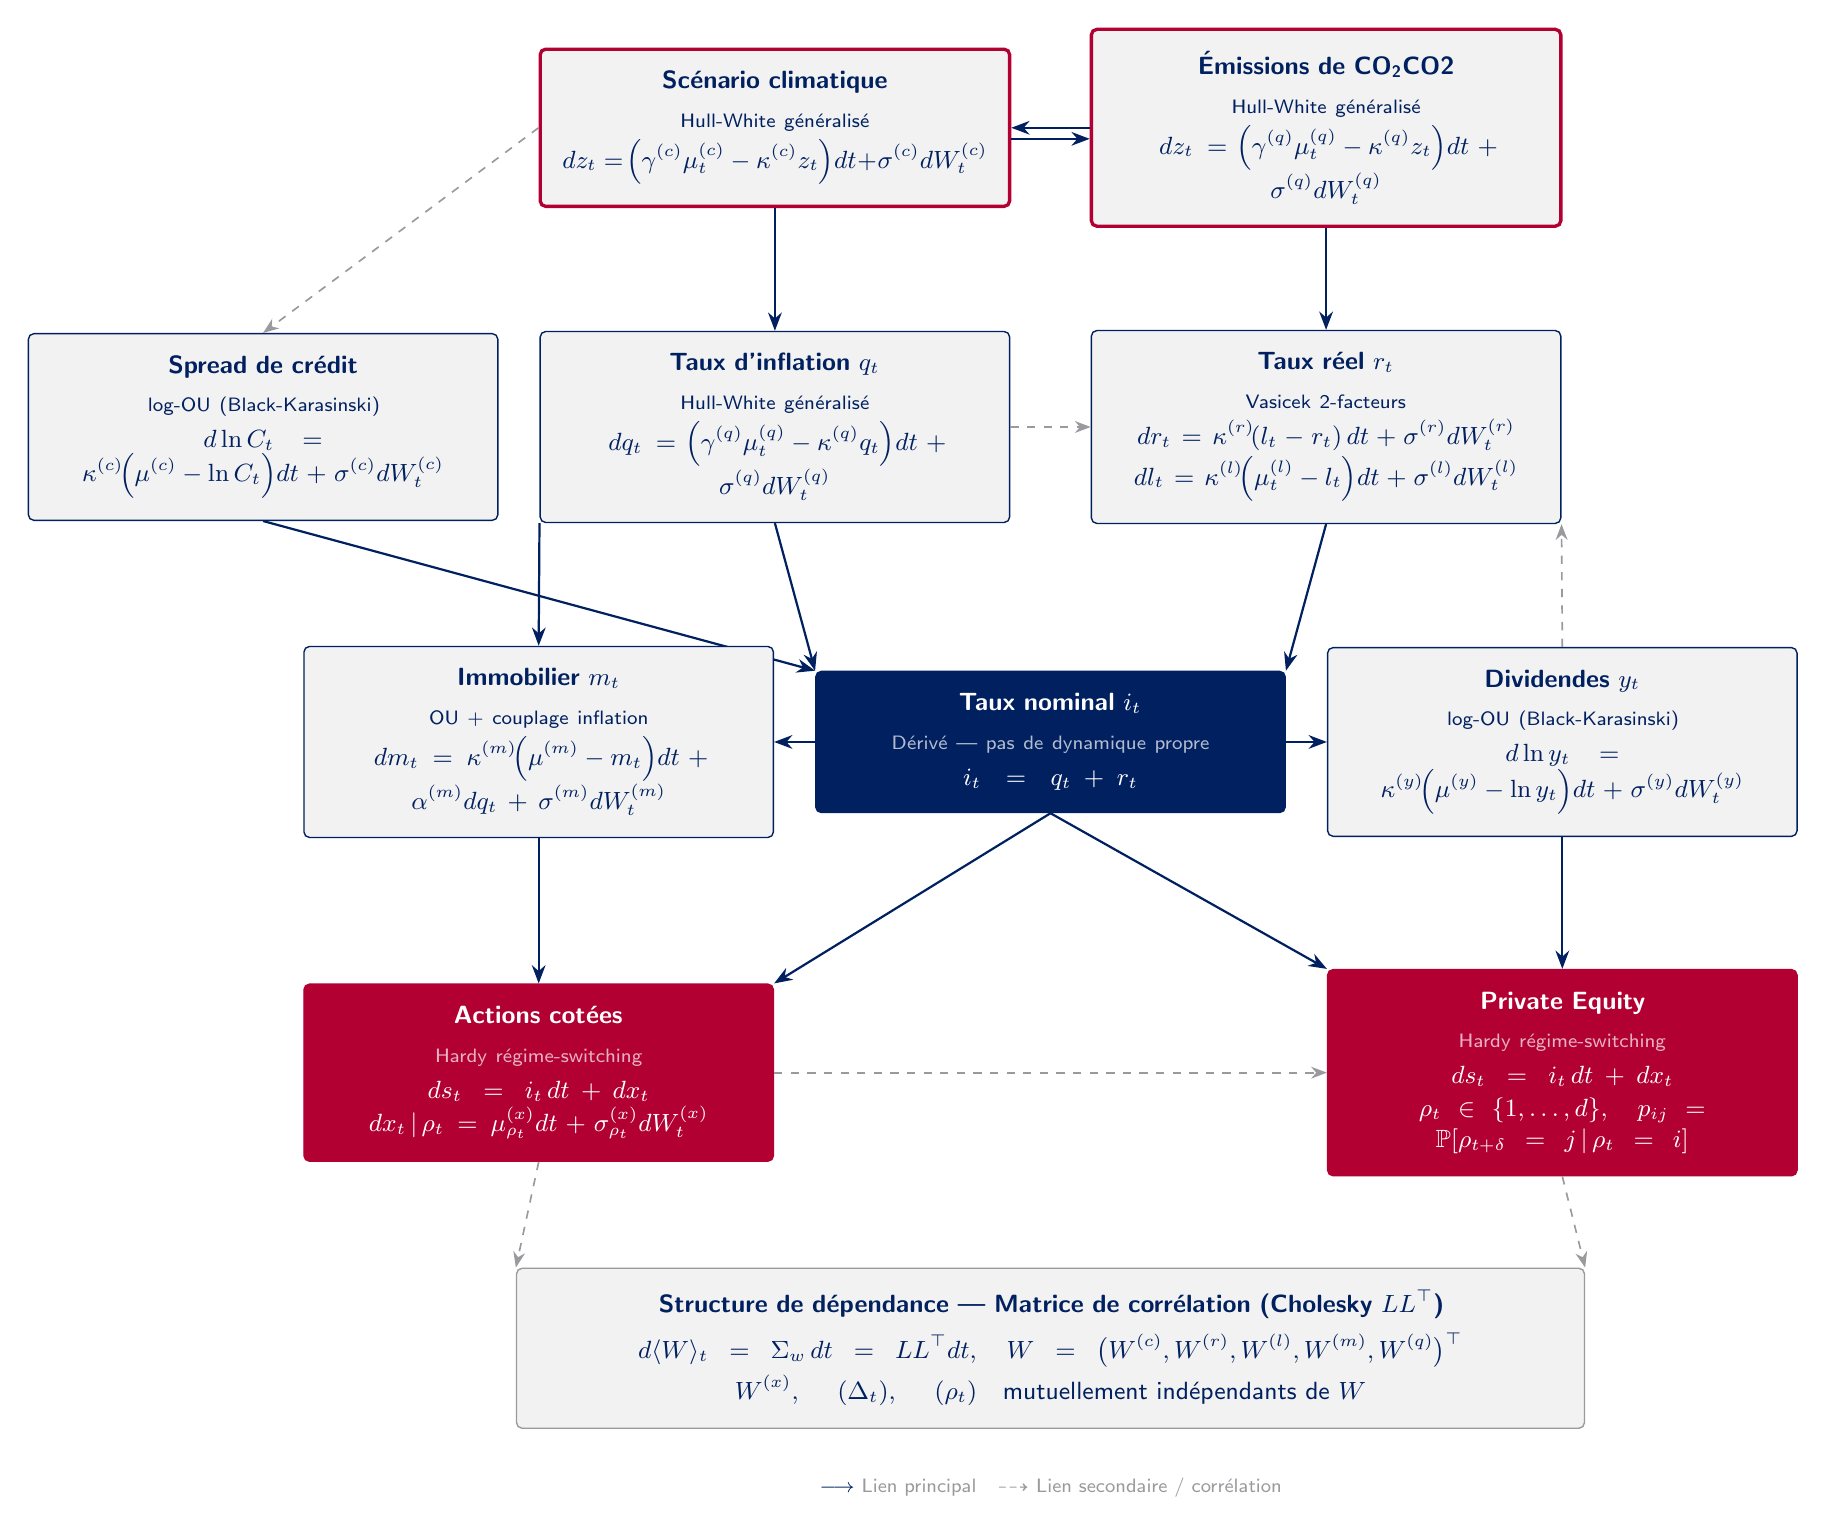
\begin{tikzpicture}[
    boite/.style={
        draw, rectangle, rounded corners=2pt, align=center,
        text width=5.4cm, inner sep=8pt,
        font=\small\sffamily, fill=nexlight, draw=nexnavy,
        text=nexnavy, line width=0.5pt
    },
    boite principal/.style={
        boite, draw=nexred, line width=1.2pt
    },
    boite pivot/.style={
        boite, fill=nexnavy, draw=nexnavy, text=white
    },
    boite sortie/.style={
        boite, fill=nexred, draw=nexred, text=white
    },
    fp/.style={-Stealth, nexnavy, line width=0.8pt},
    fs/.style={-Stealth, nexgrey, line width=0.6pt, dashed},
    >=Stealth
]

%── Niveau 1 : facteurs climatiques ────────────────────────────────────────
\node[boite principal] (scenclimat) at (0,0) {%
    {\small\bfseries\sffamily Scénario climatique}\\[3pt]
    {\scriptsize\sffamily Hull-White généralisé}\\[2pt]
    $\displaystyle dz_t = \!\left(\gamma^{(c)}\mu_t^{(c)}
      - \kappa^{(c)} z_t\right)\!dt + \sigma^{(c)} dW_t^{(c)}$
};

\node[boite principal] (emissco2) at (7,0) {%
    {\small\bfseries\sffamily Émissions de \texorpdfstring{CO\textsubscript{2}}{CO2}}\\[3pt]
    {\scriptsize\sffamily Hull-White généralisé}\\[2pt]
    $\displaystyle dz_t = \!\left(\gamma^{(q)}\mu_t^{(q)}
      - \kappa^{(q)} z_t\right)\!dt + \sigma^{(q)} dW_t^{(q)}$
};

\draw[fp] (emissco2.west)  -- (scenclimat.east);
\draw[fp] ([yshift=-4pt]scenclimat.east) -- ([yshift=-4pt]emissco2.west);

%── Spread de crédit (gauche) ───────────────────────────────────────────────
\node[boite] (spread) at (-6.5,-3.8) {%
    {\small\bfseries\sffamily Spread de crédit}\\[3pt]
    {\scriptsize\sffamily log-OU (Black-Karasinski)}\\[2pt]
    $\displaystyle d\ln C_t = \kappa^{(c)}\!\!\left(\mu^{(c)} - \ln C_t\right)\!dt
      + \sigma^{(c)} dW_t^{(c)}$
};

%── Niveau 2 : inflation et taux réel ──────────────────────────────────────
\node[boite] (inflation) at (0,-3.8) {%
    {\small\bfseries\sffamily Taux d'inflation $q_t$}\\[3pt]
    {\scriptsize\sffamily Hull-White généralisé}\\[2pt]
    $\displaystyle dq_t = \!\left(\gamma^{(q)}\mu_{t}^{(q)}
      - \kappa^{(q)} q_t\right)\!dt + \sigma^{(q)} dW_t^{(q)}$
};

\node[boite] (tauxreel) at (7,-3.8) {%
    {\small\bfseries\sffamily Taux réel $r_t$}\\[3pt]
    {\scriptsize\sffamily Vasicek 2-facteurs}\\[2pt]
    $\displaystyle dr_t = \kappa^{(r)}\!(l_t - r_t)\,dt + \sigma^{(r)} dW_t^{(r)}$\\[1pt]
    $\displaystyle dl_t = \kappa^{(l)}\!\!\left(\mu_t^{(l)} - l_t\right)\!dt + \sigma^{(l)} dW_t^{(l)}$
};

\draw[fp] (scenclimat.south) -- (inflation.north);
\draw[fp] (emissco2.south)   -- (tauxreel.north);
\draw[fs] (inflation.east)   -- (tauxreel.west);
\draw[fs] (scenclimat.west)  -- (spread.north);

%── Niveau 3 : taux nominal ────────────────────────────────────────────────
\node[boite pivot] (tauxnom) at (3.5,-7.8) {%
    {\small\bfseries\sffamily\color{white} Taux nominal $i_t$}\\[3pt]
    {\scriptsize\sffamily\color{white!70!nexnavy} Dérivé — pas de dynamique propre}\\[2pt]
    $\displaystyle i_t = q_t + r_t$
};

\draw[fp] (inflation.south)  -- (tauxnom.north west);
\draw[fp] (tauxreel.south)   -- (tauxnom.north east);
\draw[fp] (spread.south)     -- (tauxnom.north west);

%── Immobilier et dividendes ────────────────────────────────────────────────
\node[boite] (immo) at (-3,-7.8) {%
    {\small\bfseries\sffamily Immobilier $m_t$}\\[3pt]
    {\scriptsize\sffamily OU + couplage inflation}\\[2pt]
    $\displaystyle dm_t = \kappa^{(m)}\!\!\left(\mu^{(m)} - m_t\right)\!dt
      + \alpha^{(m)} dq_t + \sigma^{(m)} dW_t^{(m)}$
};

\node[boite] (div) at (10,-7.8) {%
    {\small\bfseries\sffamily Dividendes $y_t$}\\[3pt]
    {\scriptsize\sffamily log-OU (Black-Karasinski)}\\[2pt]
    $\displaystyle d\ln y_t = \kappa^{(y)}\!\!\left(\mu^{(y)} - \ln y_t\right)\!dt
      + \sigma^{(y)} dW_t^{(y)}$
};

\draw[fp] (inflation.south west) -- (immo.north);
\draw[fp] (tauxnom.west)         -- (immo.east);
\draw[fp] (tauxnom.east)         -- (div.west);
\draw[fs] (div.north)            -- (tauxreel.south east);

%── Niveau 4 : rendements d'actions ────────────────────────────────────────
\node[boite sortie] (cote) at (-3,-12) {%
    {\small\bfseries\sffamily\color{white} Actions cotées}\\[3pt]
    {\scriptsize\sffamily\color{white!70!nexred} Hardy régime-switching}\\[2pt]
    $\displaystyle ds_t = i_t\,dt + dx_t$\\[1pt]
    $\displaystyle dx_t\,|\,\rho_t = \mu^{(x)}_{\rho_t}dt
      + \sigma^{(x)}_{\rho_t} dW_t^{(x)}$
};

\node[boite sortie] (pe) at (10,-12) {%
    {\small\bfseries\sffamily\color{white} Private Equity}\\[3pt]
    {\scriptsize\sffamily\color{white!70!nexred} Hardy régime-switching}\\[2pt]
    $\displaystyle ds_t = i_t\,dt + dx_t$\\[1pt]
    $\displaystyle \rho_t \in \{1,\dots,d\},\quad
      p_{ij} = \mathbb{P}[\rho_{t+\delta}=j\,|\,\rho_t=i]$
};

\draw[fp] (tauxnom.south)  -- (cote.north east);
\draw[fp] (tauxnom.south)  -- (pe.north west);
\draw[fp] (immo.south)     -- (cote.north);
\draw[fp] (div.south)      -- (pe.north);
\draw[fs] (cote.east)      -- (pe.west);

%── Structure de dépendance (bas) ──────────────────────────────────────────
\node[boite, draw=nexgrey, text width=13cm] (correl) at (3.5,-15.5) {%
    {\small\bfseries\sffamily Structure de dépendance — Matrice de corrélation
     (Cholesky $LL^\top$)}\\[4pt]
    $\displaystyle
      d\langle W\rangle_t = \Sigma_w\,dt = LL^\top dt,
      \quad W = \bigl(W^{(c)}, W^{(r)}, W^{(l)},
                       W^{(m)}, W^{(q)}\bigr)^\top$\\[2pt]
    $\displaystyle W^{(x)},\;(\Delta_t),\;(\rho_t)
      \quad\text{mutuellement indépendants de } W$
};

\draw[fs] (cote.south) -- (correl.north west);
\draw[fs] (pe.south)   -- (correl.north east);

%── Légende ────────────────────────────────────────────────────────────────
\node[below=0.5cm of correl, font=\scriptsize\sffamily\color{nexgrey}] {
    \textcolor{nexnavy}{$\longrightarrow$} Lien principal\quad
    \textcolor{nexgrey}{$\dashrightarrow$} Lien secondaire / corrélation
};

\end{tikzpicture}%
}
\end{center}

Matar va proposer d'utiliser les paramètres prospectif de rendement pour calibrer les diffusions (contrainte de localité sur le maximum de vraisemblance) autour des rendements implicité par les assets managers ainsi que les données de marchés.

\clearpage
\appendix
\renewcommand{\thesection}{\Alph{section}}
% Annexes : même style v2 que les sections (Montserrat navy, sans filet)
\titleformat{\section}{\sffamily\Large\bfseries\color{nxnavy}}{Annexe~\thesection~-}{0.5em}{}

\section{Liste des documents et fichiers reçus}

\begin{longtable}{P{5.0cm}P{3.0cm}P{1.8cm}P{5.0cm}}
\toprule
\tablehead{Document / fichier} & \tablehead{Émetteur} & \tablehead{Date} & \tablehead{Description} \\
\midrule\endfirsthead
\toprule
\tablehead{Document / fichier} & \tablehead{Émetteur} & \tablehead{Date} & \tablehead{Description} \\
\midrule\endhead
\bottomrule\endfoot
{\small \texttt{Template\_Allocationv2.xlsm}} & {\small CDC - DPS / ALM-RF} & {\small 2025/2026} & {\small Paramètres GSE (20 / 15 ans), prime de liquidité, corrélations, sorties de simulation} \\
\rowcolor{nxlightblue}
{\small Refonte Modèle Allocation d'actifs (note)} & {\small CDC - DPS / ALM-RF} & {\small [Date]} & {\small Documentation de la refonte du GSE} \\
{\small Rapport Milliman - Revue des paramètres} & {\small Milliman} & {\small 01/07/2022} & {\small Revue indépendante précédente} \\
\rowcolor{nxlightblue}
{\small [Codes R - calibrage anciens facteurs]} & {\small [CDC]} & {\small [Date]} & {\small [À compléter]} \\
{\small [Codes Python - corrélations]} & {\small [CDC]} & {\small [Date]} & {\small [À compléter]} \\
\rowcolor{nxlightblue}
{\small [Code MATLAB - simulation]} & {\small [CDC]} & {\small [Date]} & {\small [À compléter]} \\
\end{longtable}
\vspace{-10pt}
\tabcaption{Inventaire des éléments transmis}

\section{Description des tests statistiques}
\ph{[Détailler : hypothèses nulles, statistiques, lois asymptotiques, limites (Shapiro-Wilk, Jarque-Bera, Ljung-Box), construction des QQ-plots, estimateur non biaisé de la variance en présence d'autocorrélation, bootstrap des intervalles de confiance.]}

\section{Protocole de réplication indépendante}
\ph{[Décrire : ré-implémentation des modèles par Nexialog, jeux de données, environnement (R / Python / MATLAB), comparaison paramètre par paramètre avec la production, tolérances, gestion des écarts.]}

\section{Glossaire}
\ph{[GSE, ALM, V2F, RSLN-2, CIR, BK, BEIR, OAT / OATi, ZC, unsmoothing, copule gaussienne, condition de Feller, schéma d'Alfonsi, SDP / Higham, etc.]}

\section{Références}
\begin{itemize}
  \item Ahlgrim, K. C., D'Arcy, S. P., \& Gorvett, R. W. (2005). \textit{Modeling financial scenarios: A framework for the actuarial profession}.
  \item Alfonsi, A. (2005). \textit{On the discretization schemes for the CIR (and Bessel squared) processes}.
  \item Hardy, M. (2001). \textit{A Regime-Switching Model of Long-Term Stock Returns}. North American Actuarial Journal.
  \item Higham, N. J. (1988). \textit{Computing a nearest symmetric positive semidefinite matrix}.
  \item Hull, J., \& White, A. (1994). \textit{Numerical procedures for implementing term structure models II}.
  \item Lizieri, C., Satchell, S., \& Wongwachara, W. (2012). \textit{Unsmoothing Real Estate Returns: A Regime-Switching Approach}.
  \item \ph{[Compléter : Milliman (2022), notes internes CDC, indicateurs de cycle DG Trésor.]}
\end{itemize}

\section{Mentions légales}
\copyright~Nexialog Consulting, \ph{2026}. Tous droits réservés. Document confidentiel fourni dans le cadre exclusif de la mission visée en page de garde. Toute reproduction ou diffusion requiert l'autorisation écrite préalable de Nexialog Consulting.

\end{document}